% Лабораторная работа по АСиСу № 11
% Михедов Константин Константинович

% Тип документа: статья, на бумаге А4
\documentclass[a4paper]{article}

% Подключение сторонних tex файлов 
\usepackage{import}


% Основные данные - ВУЗ, факультет, город...
\import{./../../stuff/tex}{config.tex}

% Подключение необходимых зависимостей
\import{./../../stuff/tex/settings}{packages.tex}
% Настройка подключенных пакетов
\import{./../../stuff/tex/settings}{preferences.tex}


% Шаблон титульной страницы 
\import{./../../stuff/tex/templates}{title.tex}
% Упрощенный блок "выполнил"
\import{./../../stuff/tex/templates}{sign1.tex}
% Макрос для содержания
\import{./../../stuff/tex/templates}{toc.tex}

% Определяем название документа
\title{
  Домашняя работа по курсу \\
  <<Системы и сети передачи информации>>  
}
% Отключаем отображение правительства
\renewcommand{\government}{}
% Отключаем сокращенное нзавание университета
\renewcommand{\subuniversity}{}
% Указываем преподавателя
\renewcommand{\shortteachername}{Банков Д.В.}


% Путь до внешних изображений
\graphicspath{ {./figures/}}


% Основной текст работы
\begin{document}
  \templatedtitlepage
  \toc

  \section{Рассчёт варианта}
  По заданию номером варианта необходимо считать остаток от деления суммы индексов первых букв
  имени и фамилии на 30.

  Моя фамилия - <<Дуников>>. Первая буква - <<Д>>. Это пятая буква русского алфавита, следовательно её индекс равен 4.
  Аналогично имя - <<Константин>>. Первая буква - <<К>>. Она является двенадцатой буквой в русском алфавите,
  поэ-тому ее индекс равен 11.

  \begin{equation}
    (4 + 11) \mod 30 = 15
  \end{equation}

  Номер вариант, исходя из общей формула рассчёта, равен 15. Для него в задании указан следующий список хостов:
  \begin{enumerate}
    \item \href{opera.com}{opera.com}
    \item \href{www.ubuntu.ru}{www.ubuntu.ru}
    \item \href{www.vlc.ru}{www.vlc.ru}
  \end{enumerate}

  \newpage
  \section{Определение параметров сетевых интерфейсов}

  Для этого обычно используется утилита \textbf{ip}. У меня на MacOS такая тоже оказалась, но,
  судя по статьям в сети, немного урезанная. Вот она:
  \begin{figure}[H]
    \centering
    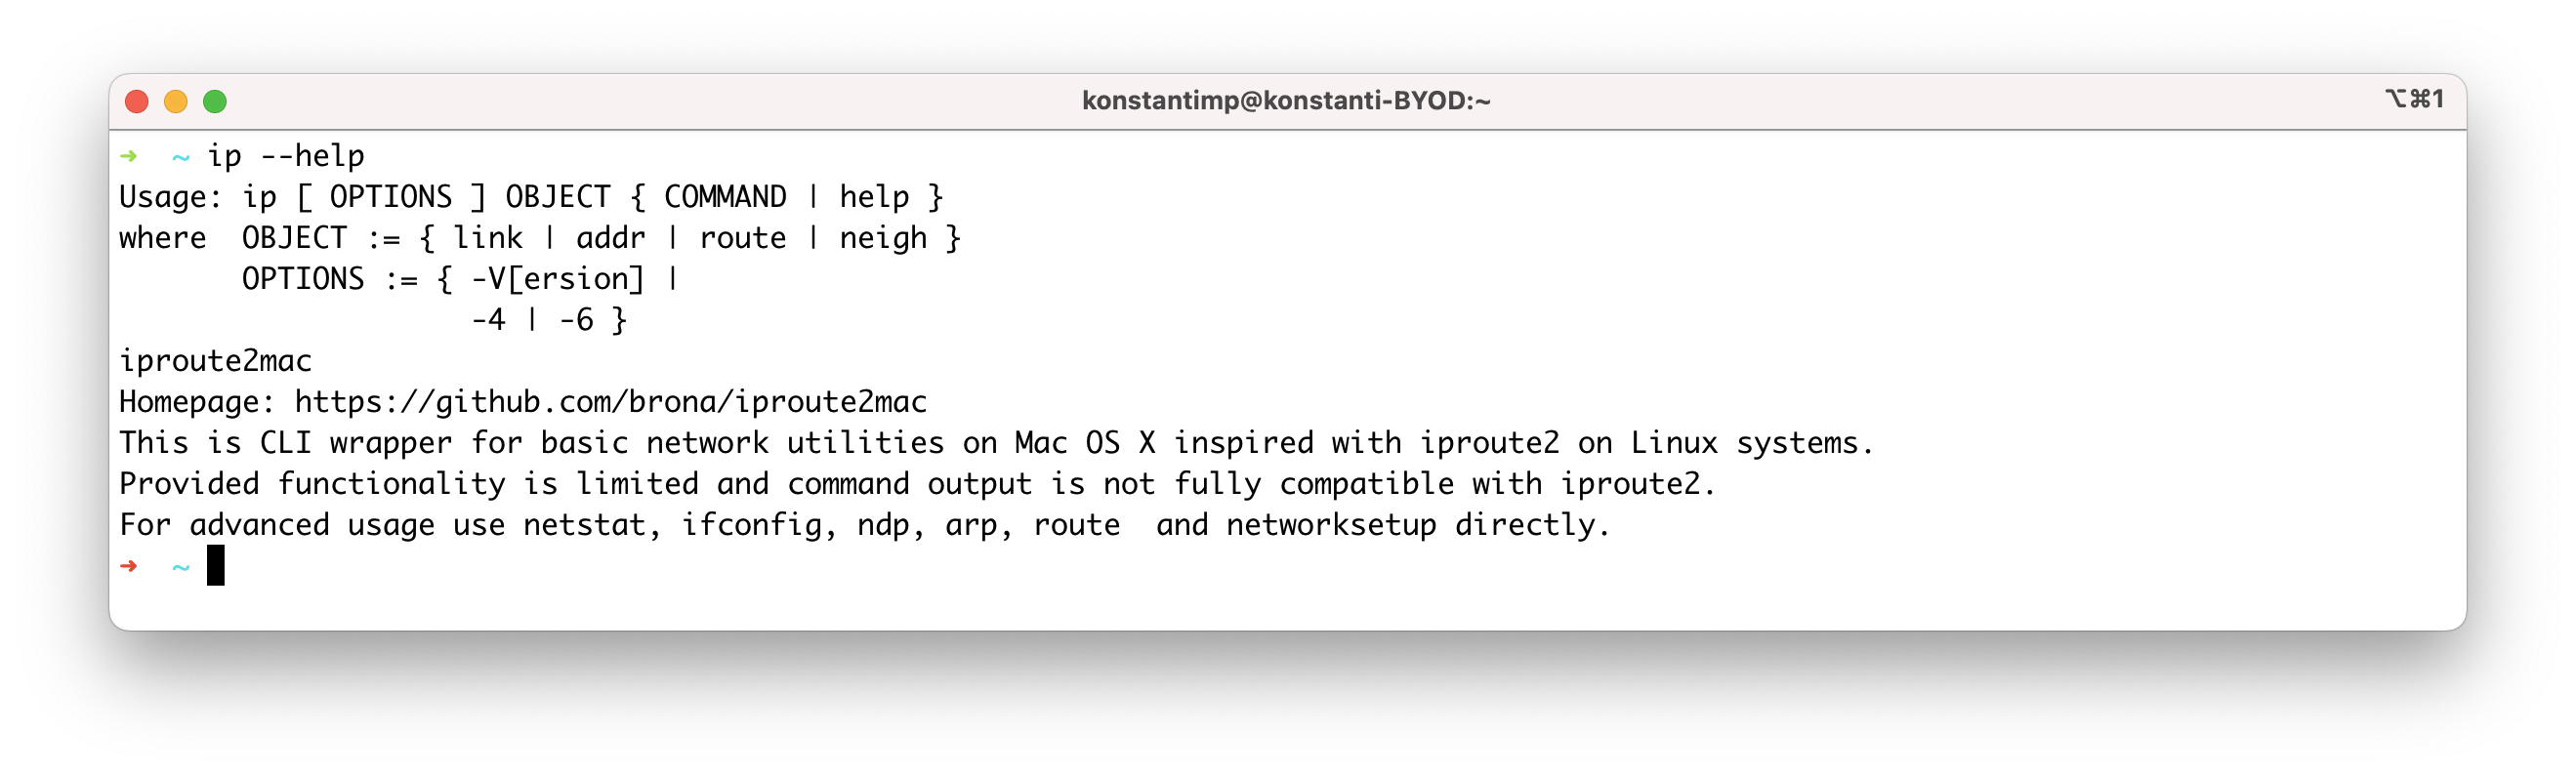
\includegraphics[width=0.8\textwidth]{s21}
    \caption{Утилита \textbf{ip}}
  \end{figure}

  Теперь с её помощью можно увидеть информацию о всех присутствующих в системе сетевых интерфейсов.
  Для этого нужно выполнить следующую команду:
  \mint{bash}|ip addr show|
  Или в более короткой форме просто
  \mint{bash}|ip a|
  \begin{figure}[H]
    \centering
    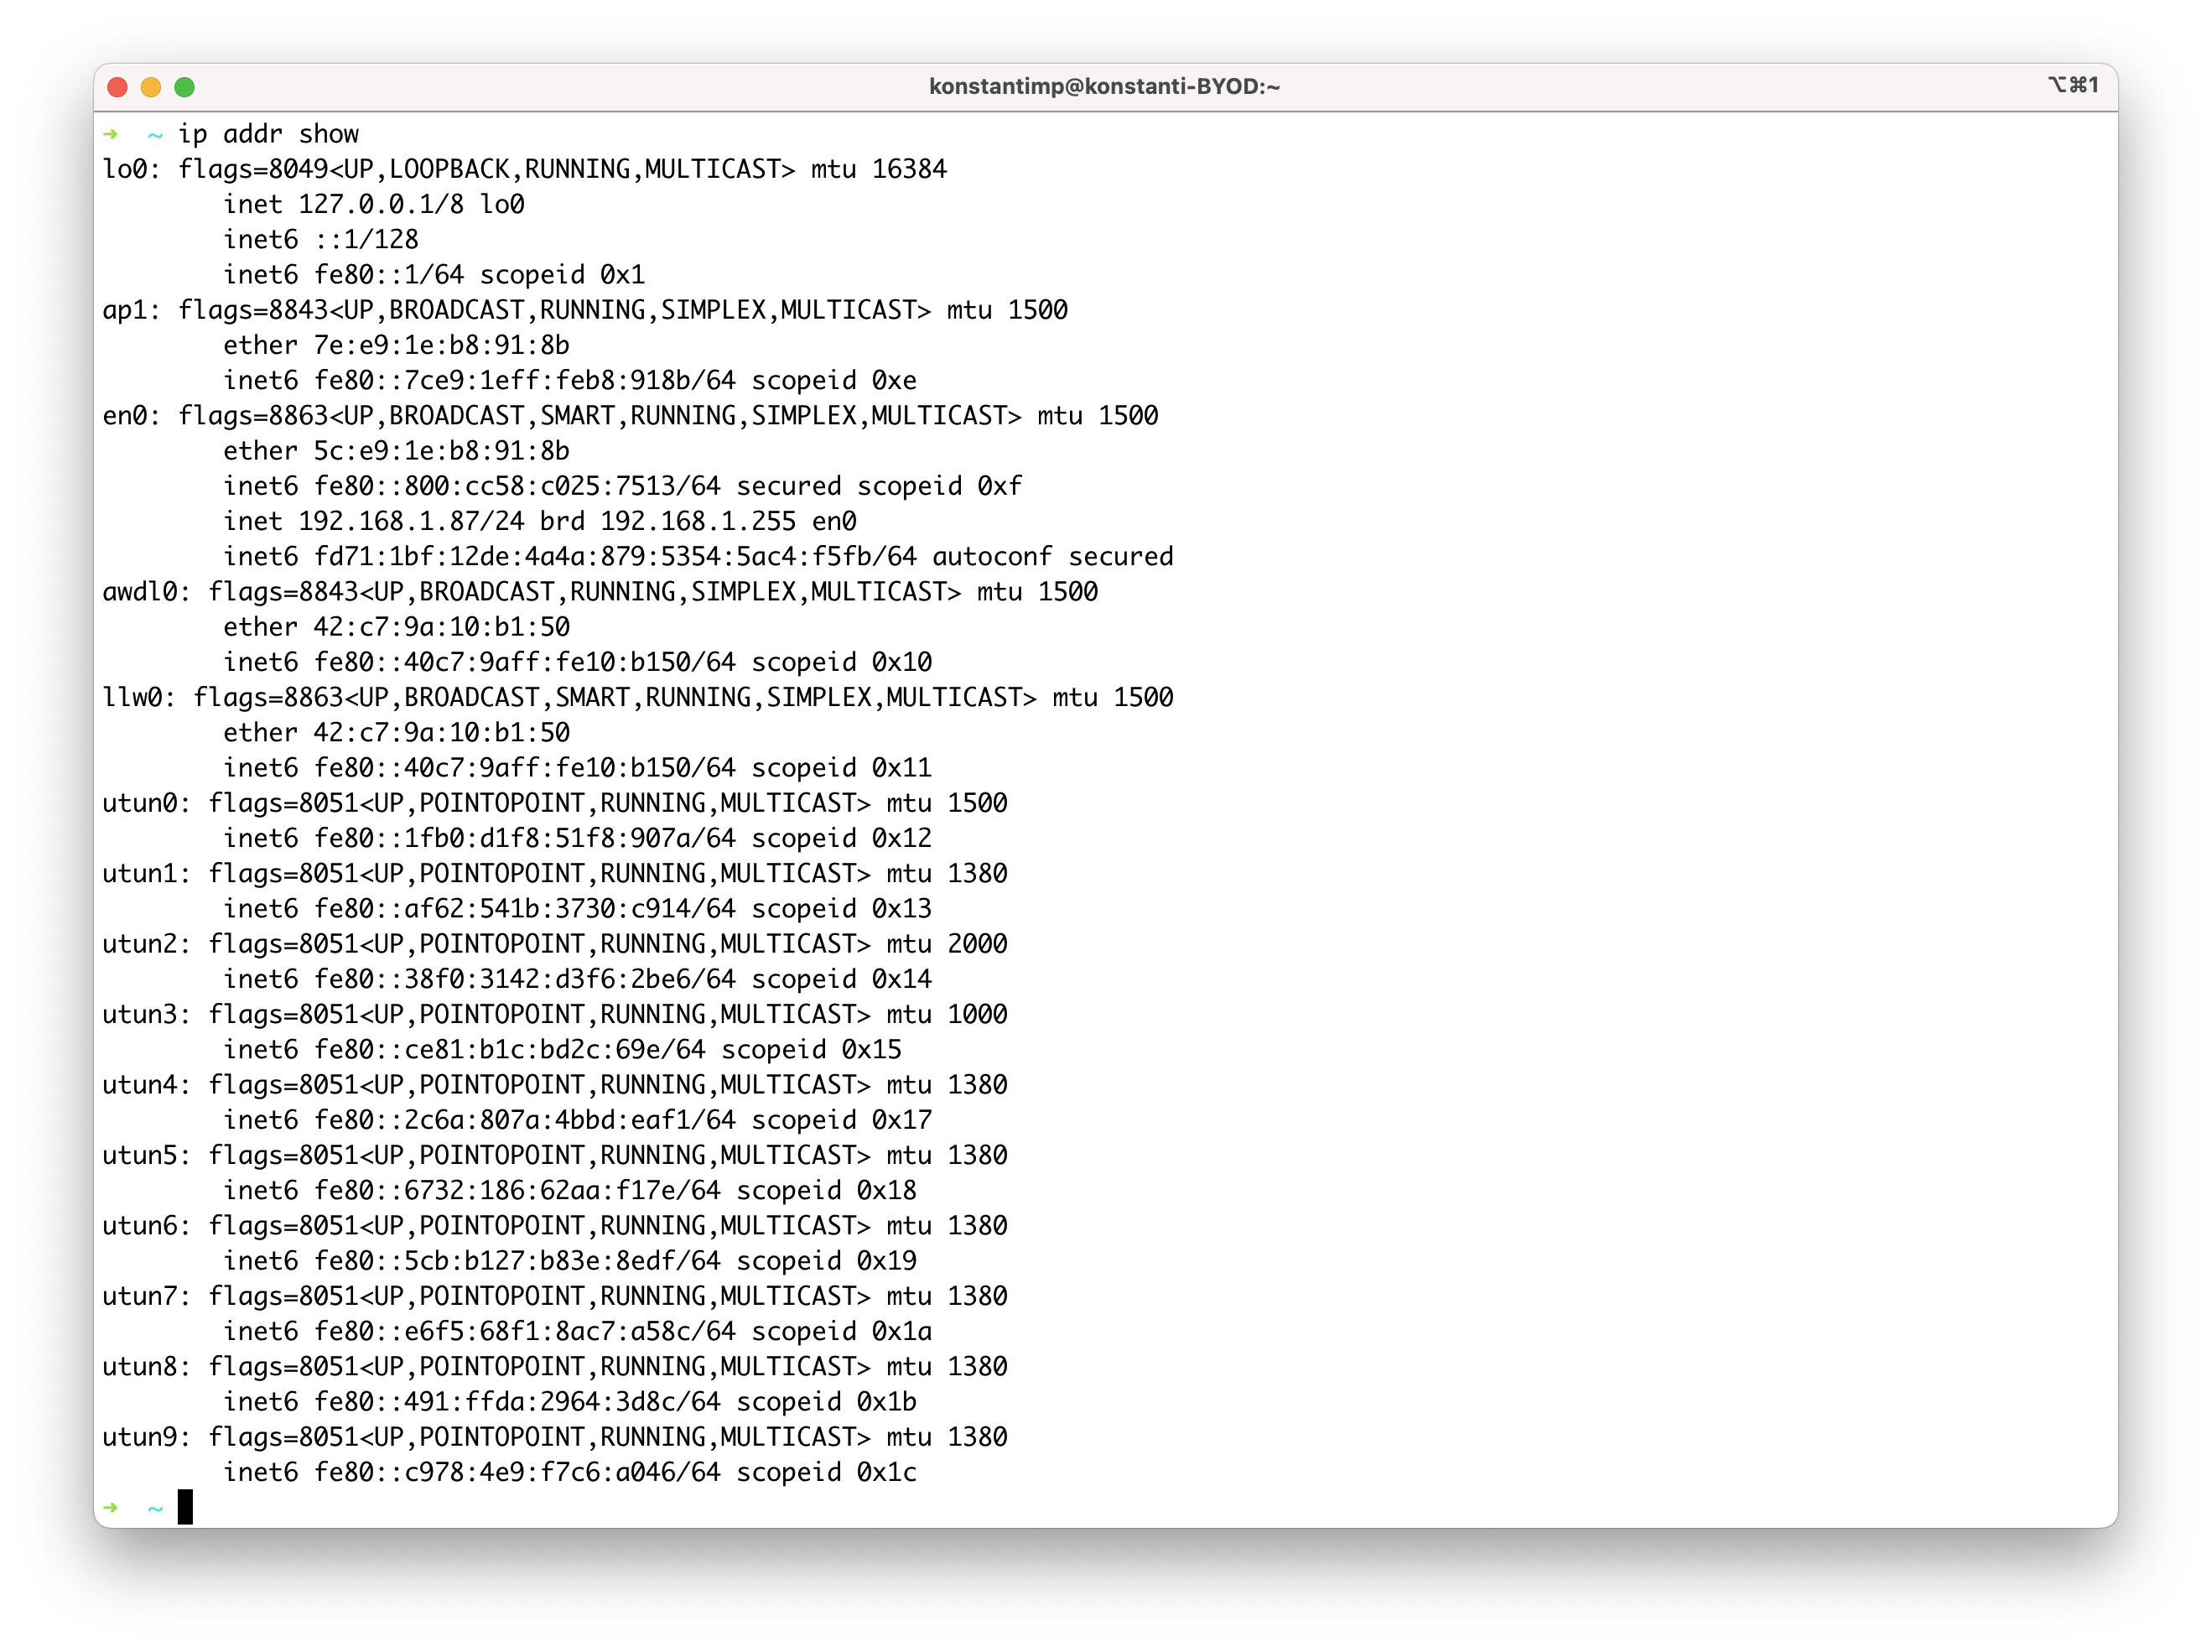
\includegraphics[width=0.8\textwidth]{s22}
    \caption{Смотрим сетевые интерфейсы}
  \end{figure}

  Что можно найти в моих сетевых интерфейсах
  \begin{itemize}
    \item {
      Много \textbf{tun} интерфейсов

      Это туннели, часть из них создана для работы VPN (у меня их WireGuard и OpenVPN, не считая сторонних приложений),
      другая часть - для связи с приложениями запущенными внутри контейнеров (Docker и Podman) и виртуальных машин (QEMU).
      Сейчас особо интереса не представляют.
    }
    \item {
      \textbf{awdl} и \textbf{llw}

      Какие-то Apple-specific устройства, которые нужны для AirDrop, AirPlay и т.п. Также нам не особо интересны
    }
    \item {
      \textbf{ap}

      Access Point - девайс, работающий как точка доступа для других устройств. Также нам не интересен
    }
    \item {
      \textbf{lo}

      Loopback - интерфейс, отправляющий пакеты обратно на мой компьютер, судя по адресу - localhost.
      Интереса сейчас не предстваляет
    }
    \item {
      \textbf{en}

      Ethernet интерфейс, через который осуществляется доступ в сеть. Он-то нам и нужен. По его параметрам
      сразу виден мой \textbf{IPv4} адрес внутри локаль-ной сети - 192.168.1.87. Отсюда также можно вытащить
      маску подсети, 255.255.255.0, и \textbf{MAC}, 5c:e9:1e:b8:91:8b.
    }
  \end{itemize}

  \newpage
  \section{Пингуем сервера}

  Чтобы проверить доступность сервера (относительно клиента), можно отправить ему несколько \textbf{ICMP} пакетов и посмотреть,
  на какое количество из них придёт ответ. Этим занимается утилита \textbf{ping}, вот она
  \begin{figure}[H]
    \centering
    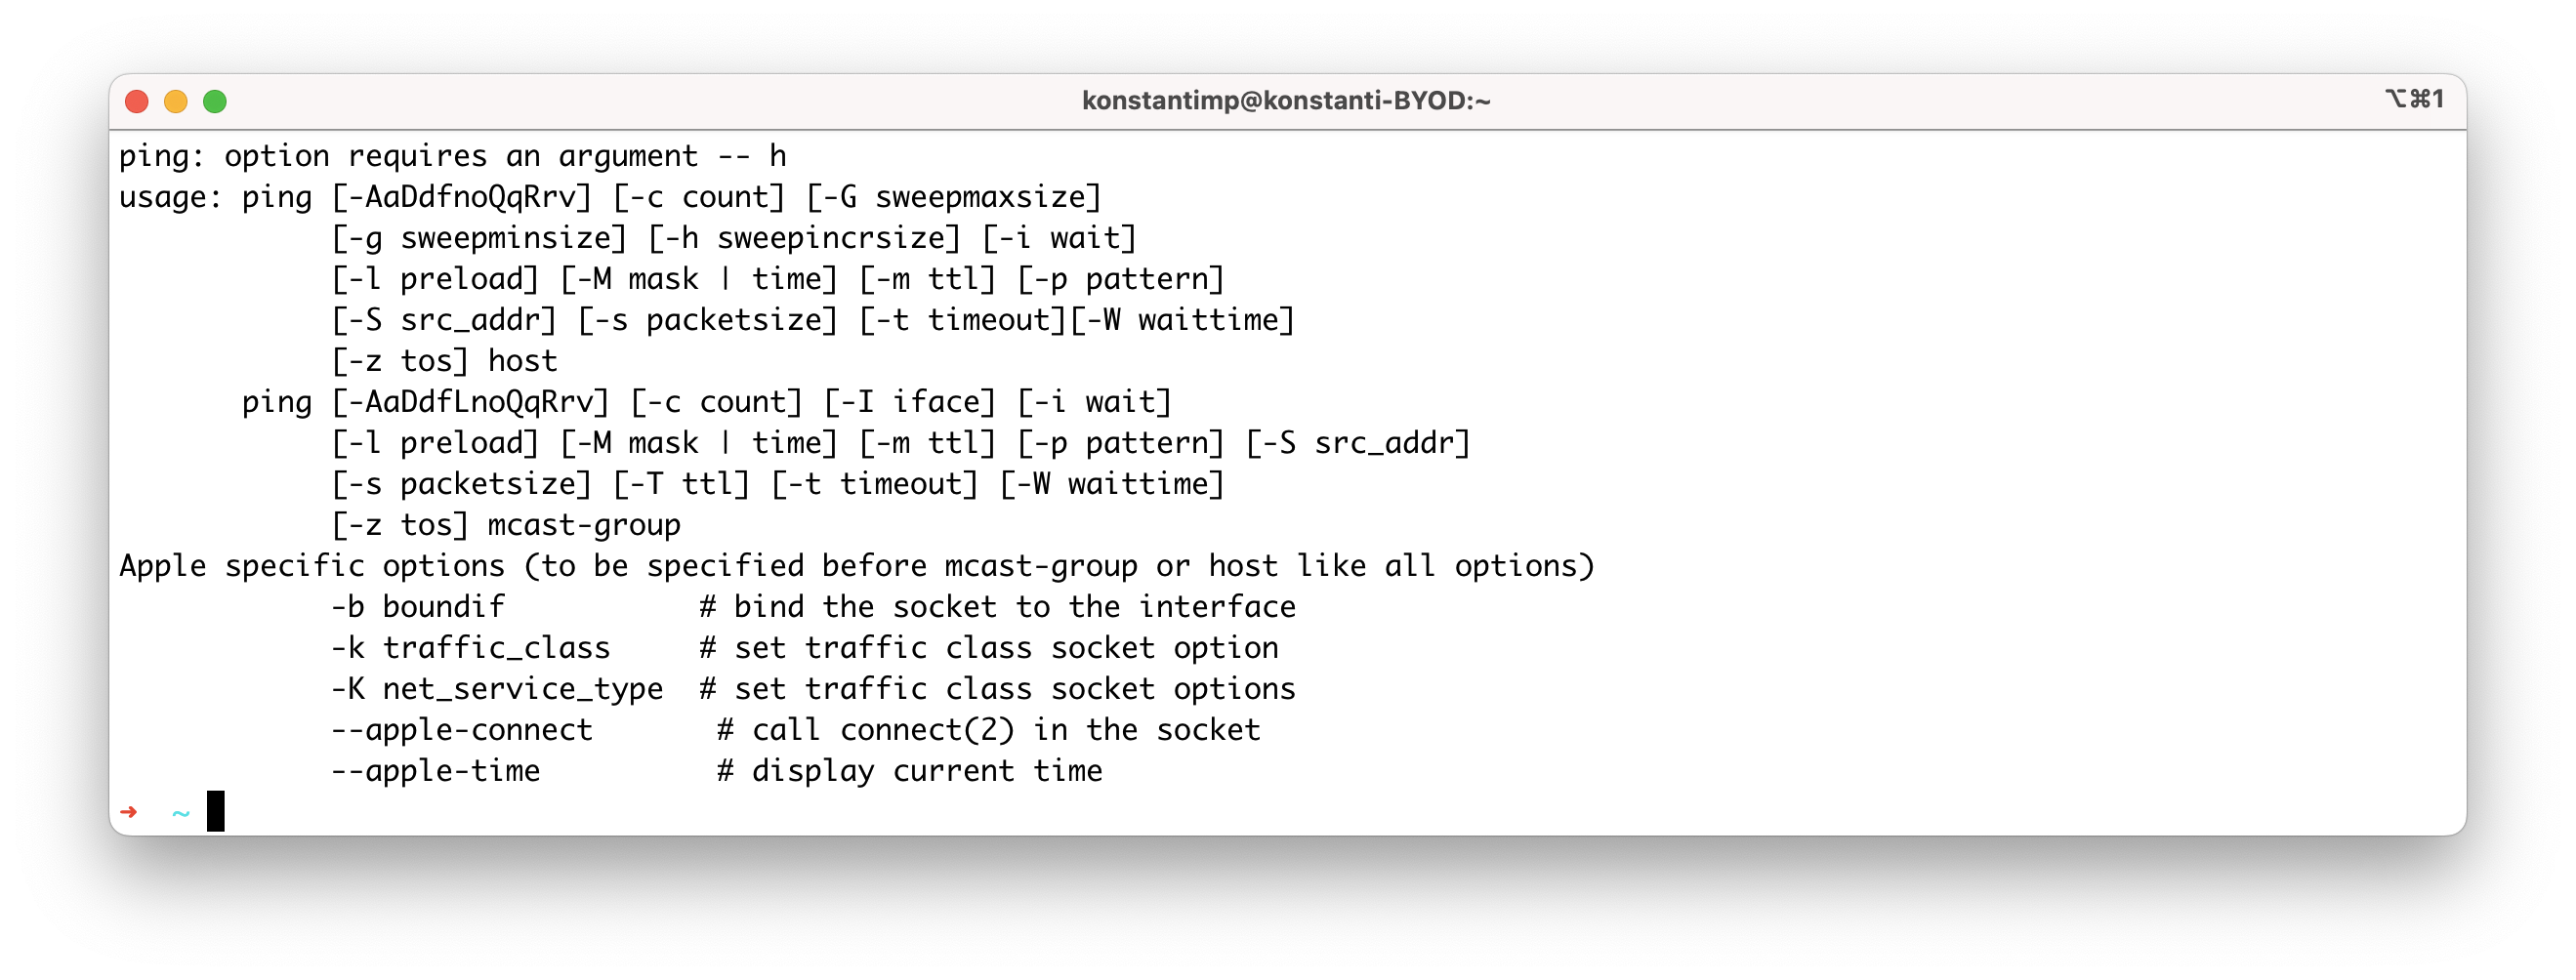
\includegraphics[width=0.8\textwidth]{s23}
    \caption{Утилита \textbf{ping}}
  \end{figure}

  Необходимо отправить по 4 echo пакета на каждый хост, для этого можно воспользоваться командой
  \mint{bash}|ping -c 4 host|
  
  \begin{figure}[H]
    \centering
    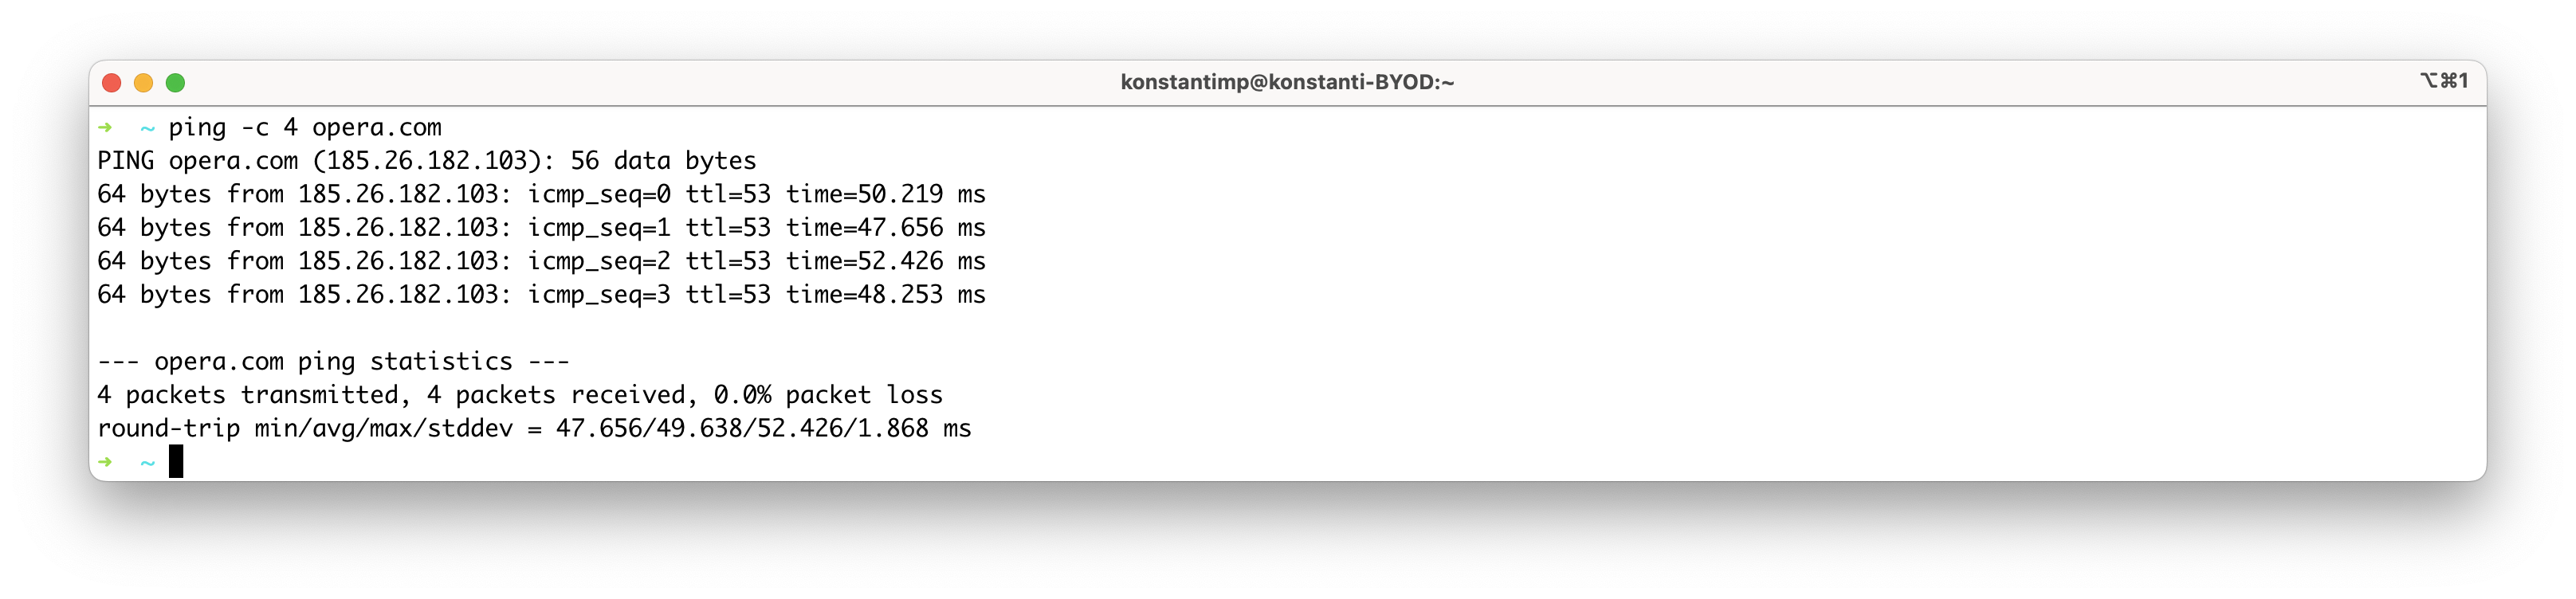
\includegraphics[width=0.8\textwidth]{s24}
    \caption{Пингуем \href{opera.com}{opera.com}}
  \end{figure}
  \begin{figure}[H]
    \centering
    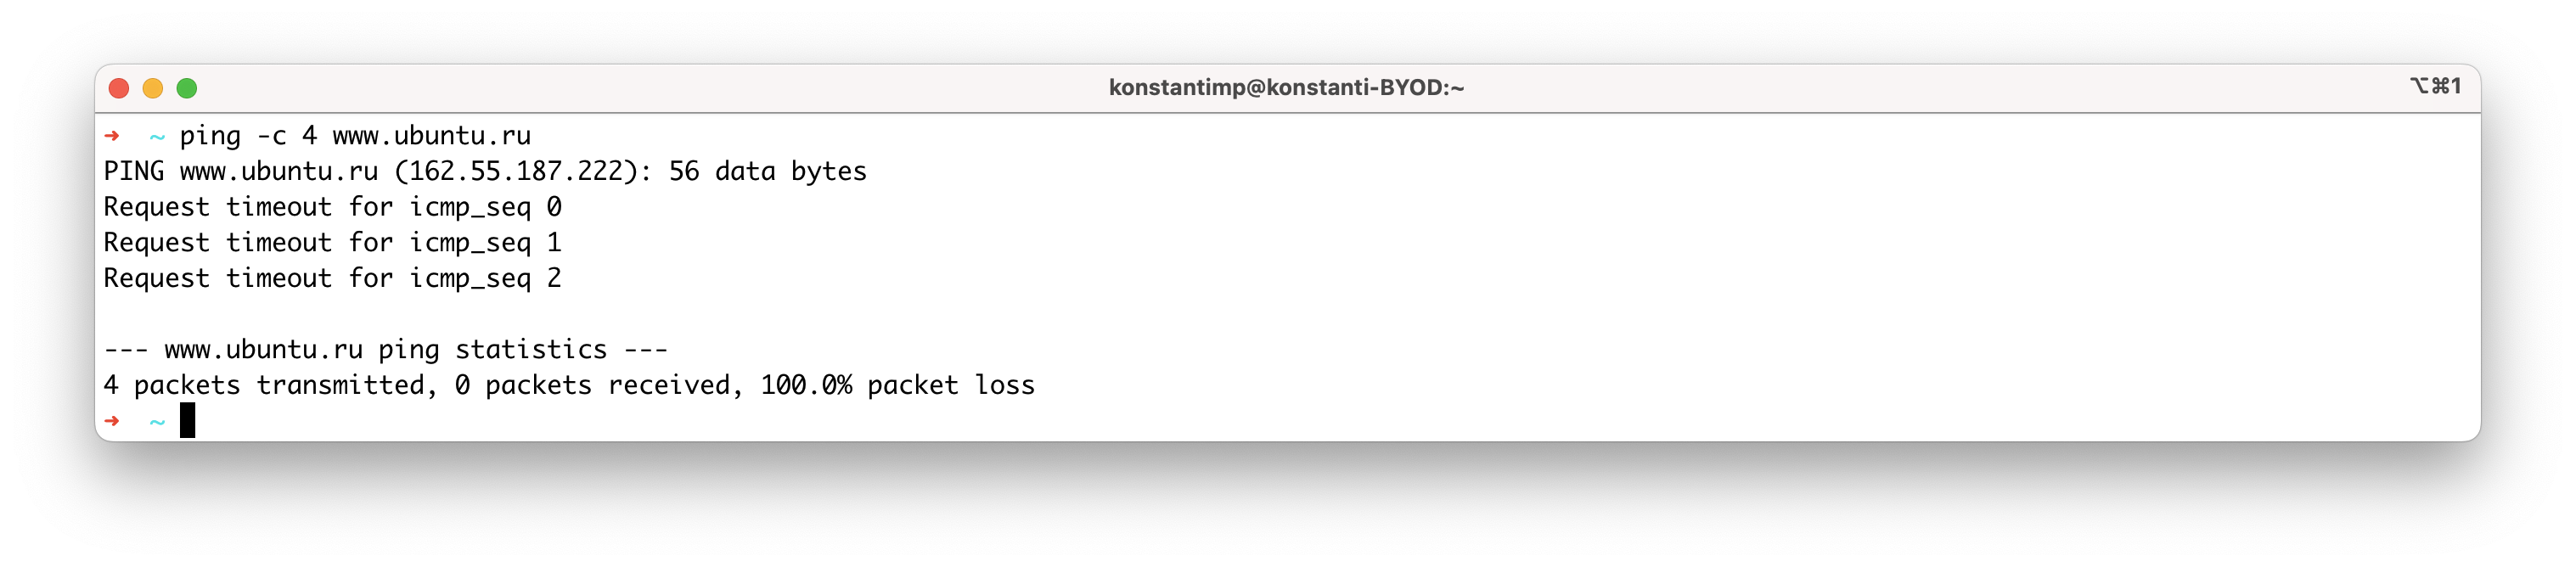
\includegraphics[width=0.8\textwidth]{s25}
    \caption{Пингуем \href{www.ubuntu.ru}{www.ubuntu.ru}}
  \end{figure}
  \begin{figure}[H]
    \centering
    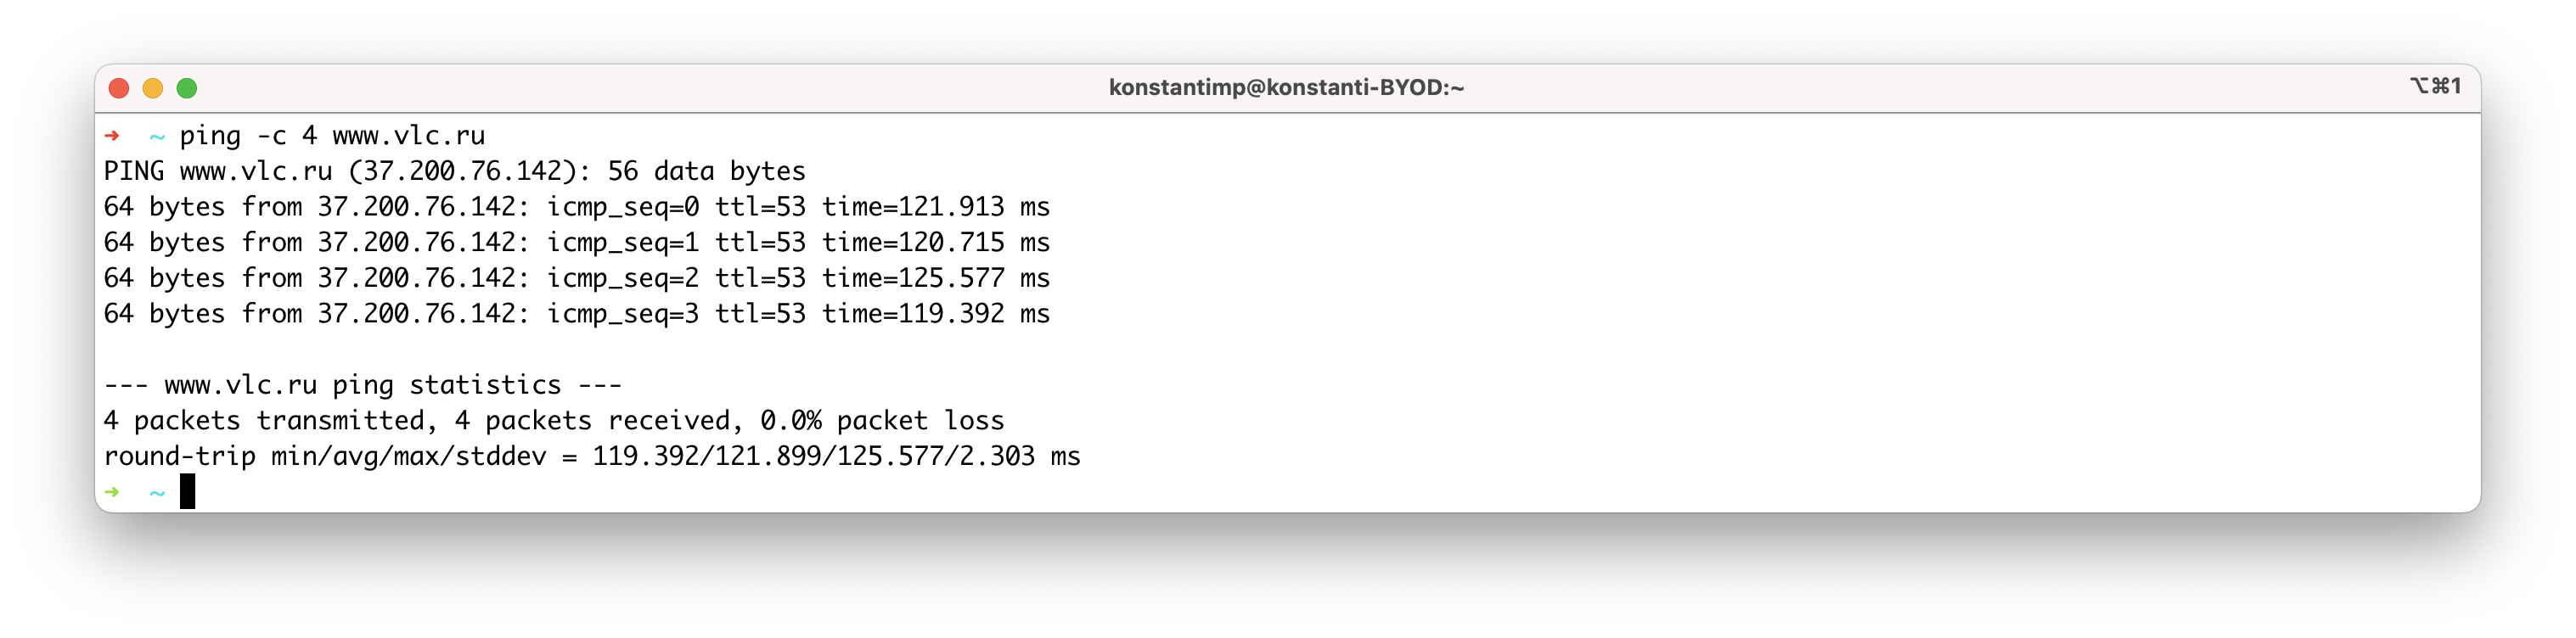
\includegraphics[width=0.8\textwidth]{s26}
    \caption{Пингуем \href{www.vlc.ru}{www.vlc.ru}}
  \end{figure}

  И вроде как всё хорошо, но \href{www.ubuntu.ru}{www.ubuntu.ru} так ни разу и не ответил. Заме-ним его на \href{www.tiktok.com}{www.tiktok.com}
  \begin{figure}[H]
    \centering
    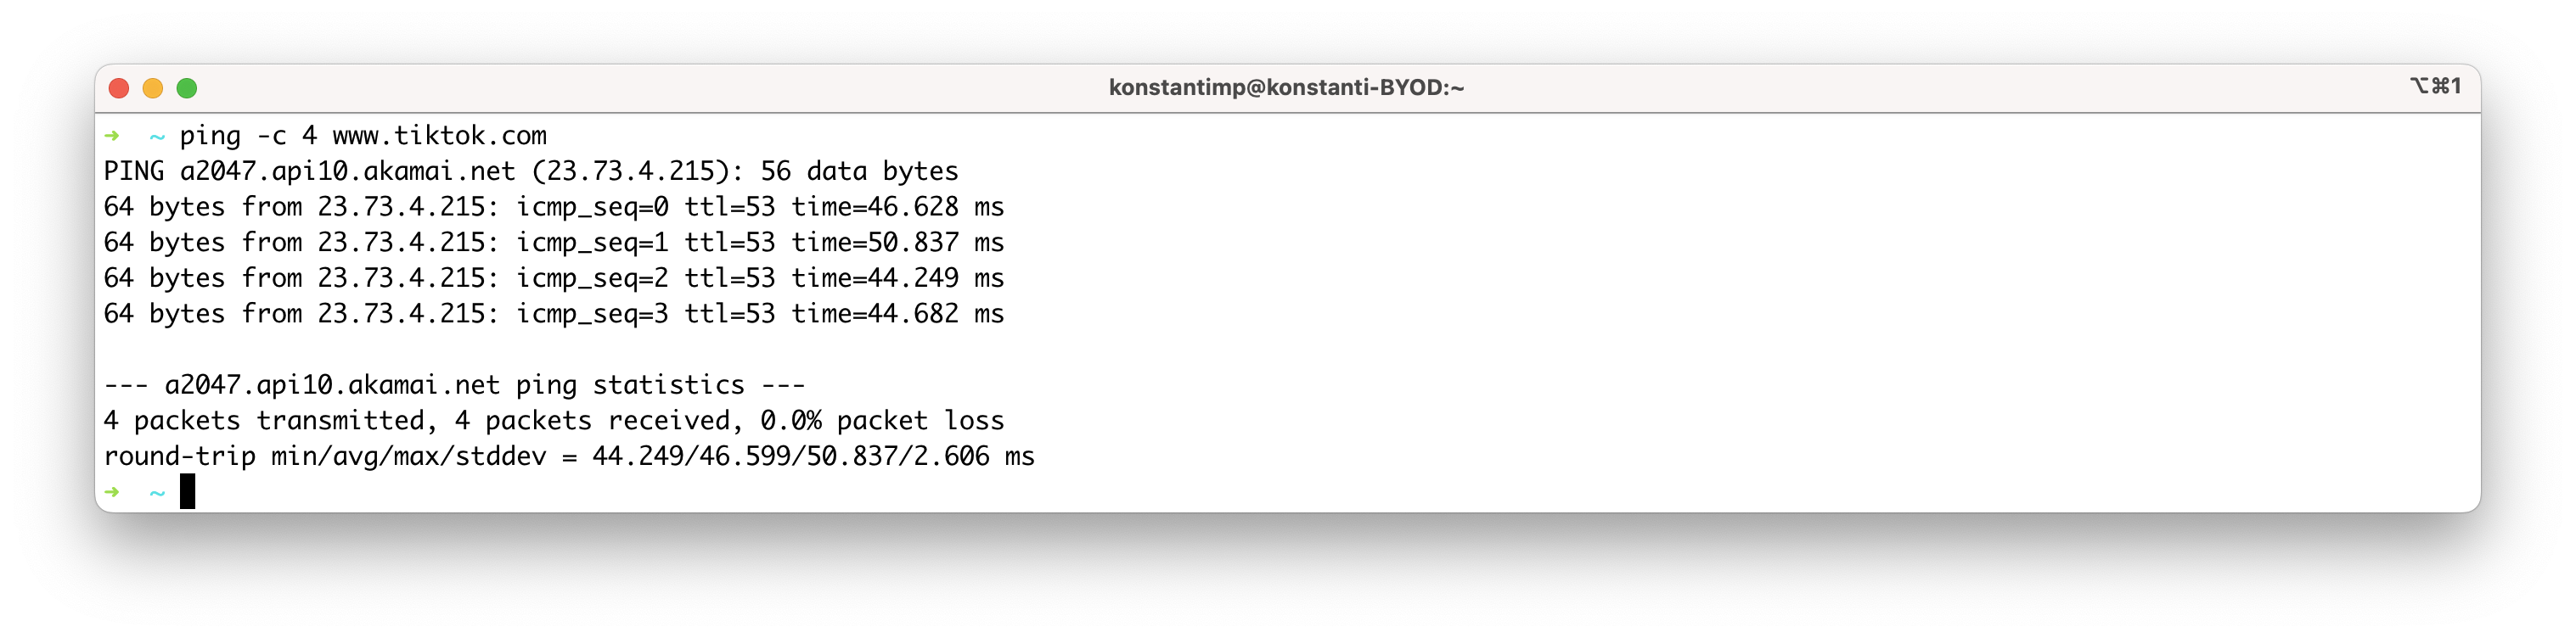
\includegraphics[width=0.8\textwidth]{s27}
    \caption{Пингуем \href{www.tiktok.ru}{www.tiktok.ru}}
  \end{figure}

  \begin{table}[H]
    \centering
    \begin{tabular}{|c|c|c|c|c|}
      \hline
      Domain Name & IP & Lost & Average Completion Time & TTL \\
      \hline
      \href{opera.com}{opera.com} & 185.26.182.103 & 0 & 49.638ms & 53 \\
      \hline
      \href{www.ubuntu.ru}{www.ubuntu.ru} & 162.55.187.222 & 4 & - & - \\
      \hline
      \href{www.vlc.ru}{www.vlc.ru} & 37.200.76.142 & 0 & 121.899ms & 53 \\
      \hline
      \href{www.tiktok.com}{www.tiktok.com} & 23.73.4.215 & 0 & 46.599ms & 53 \\
      \hline
    \end{tabular}
    \caption{В общих чертах}
  \end{table}

  \newpage
  \section{Следим за пакетом}

  Можно отследить, каким путём пакет доходит до пункта назначения, для этого есть утилита \textbf{traceroute}
  \begin{figure}[H]
    \centering
    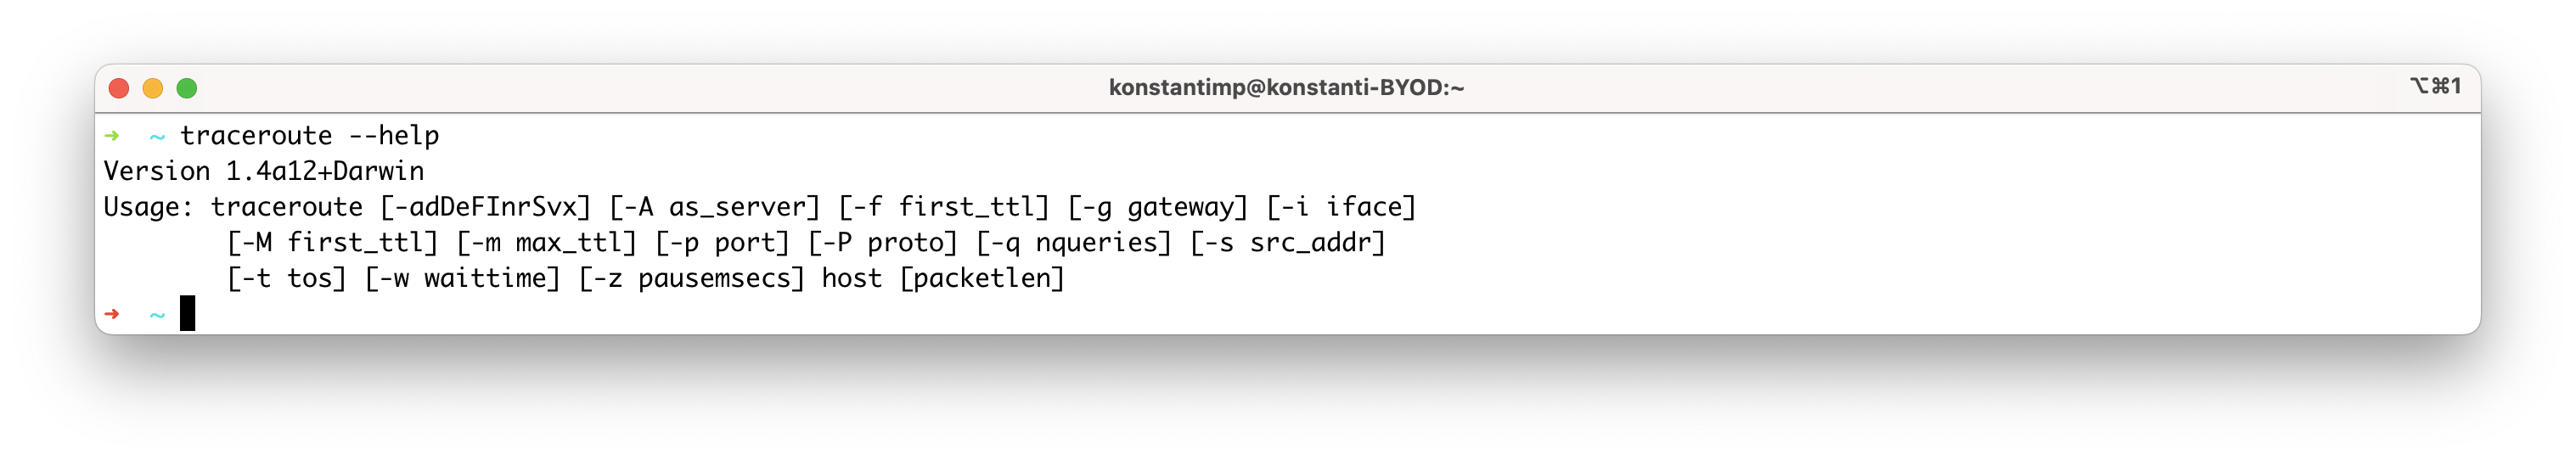
\includegraphics[width=0.8\textwidth]{s28}
    \caption{Утилита \textbf{tarceroute}}
  \end{figure}

  Синтаксис для просмотра пути (трейса) очень прост
  \mint{bash}|traceroute host|
  
  \begin{figure}[H]
    \centering
    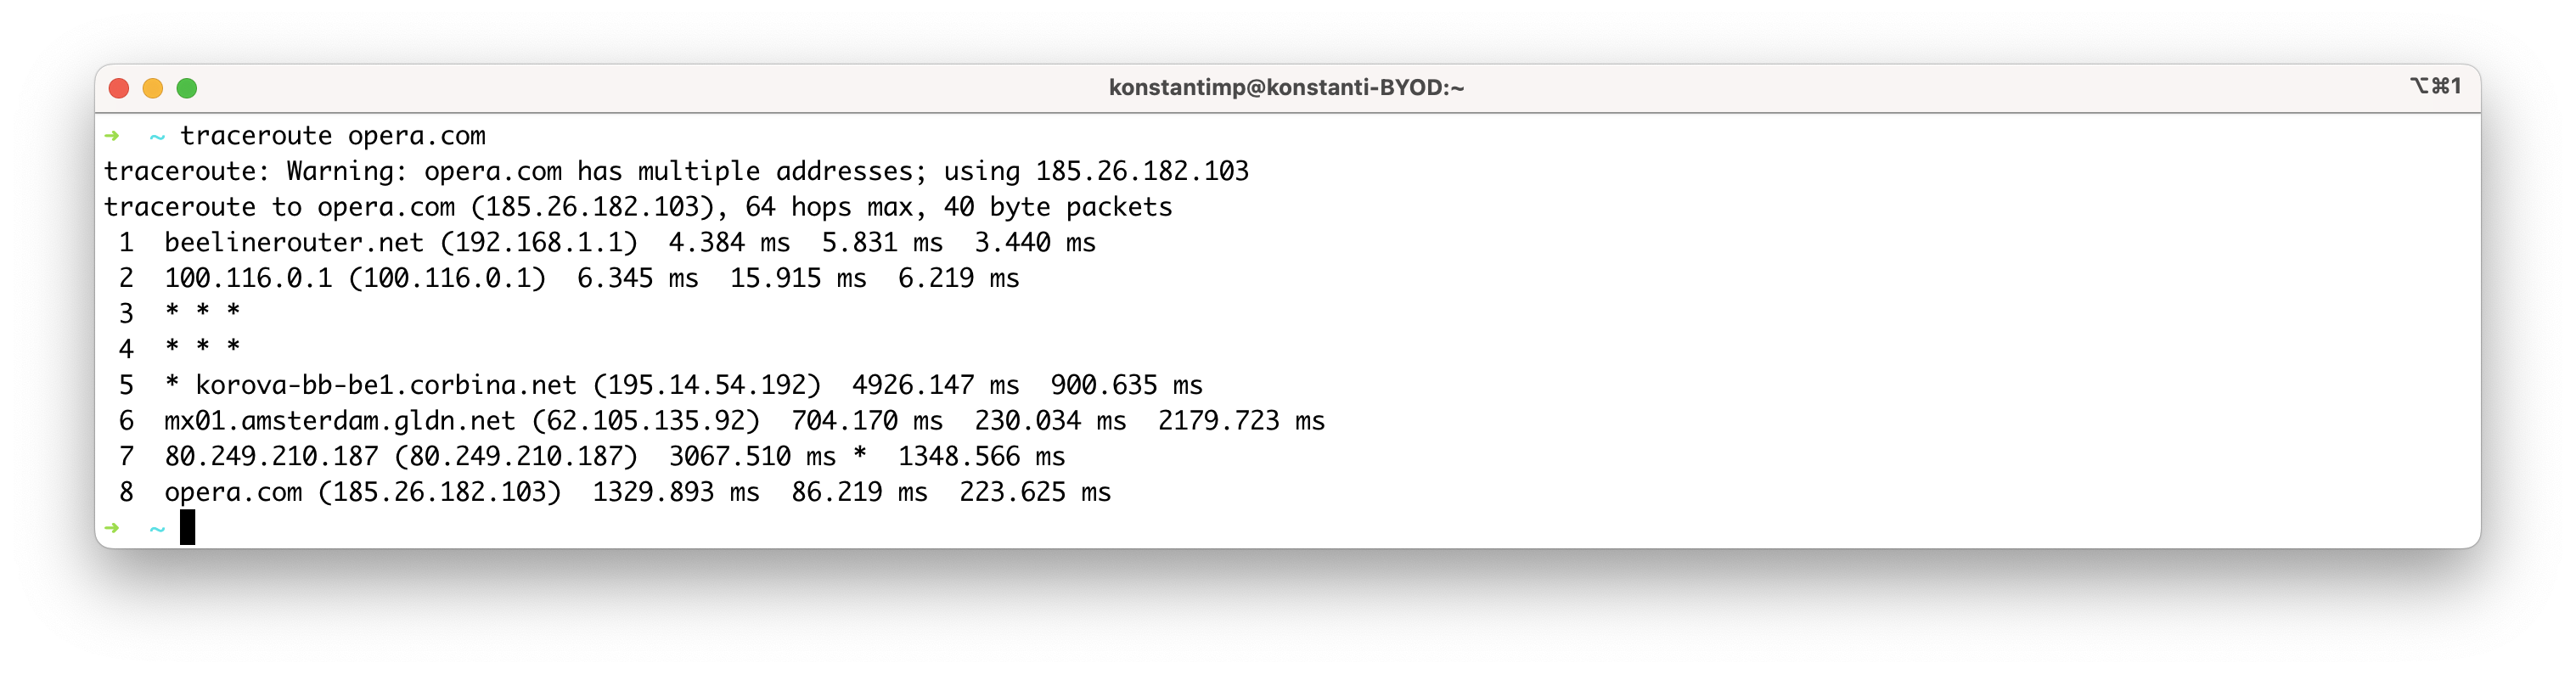
\includegraphics[width=0.8\textwidth]{s29}
    \caption{Смотрим путь пакета до \href{opera.com}{opera.com}}
  \end{figure}

  Всего 7 промежуточных узлов, наиболее долго пакеты проходили для 6 и 7 (там время получения ответа максимально).
  
  \begin{figure}[H]
    \centering
    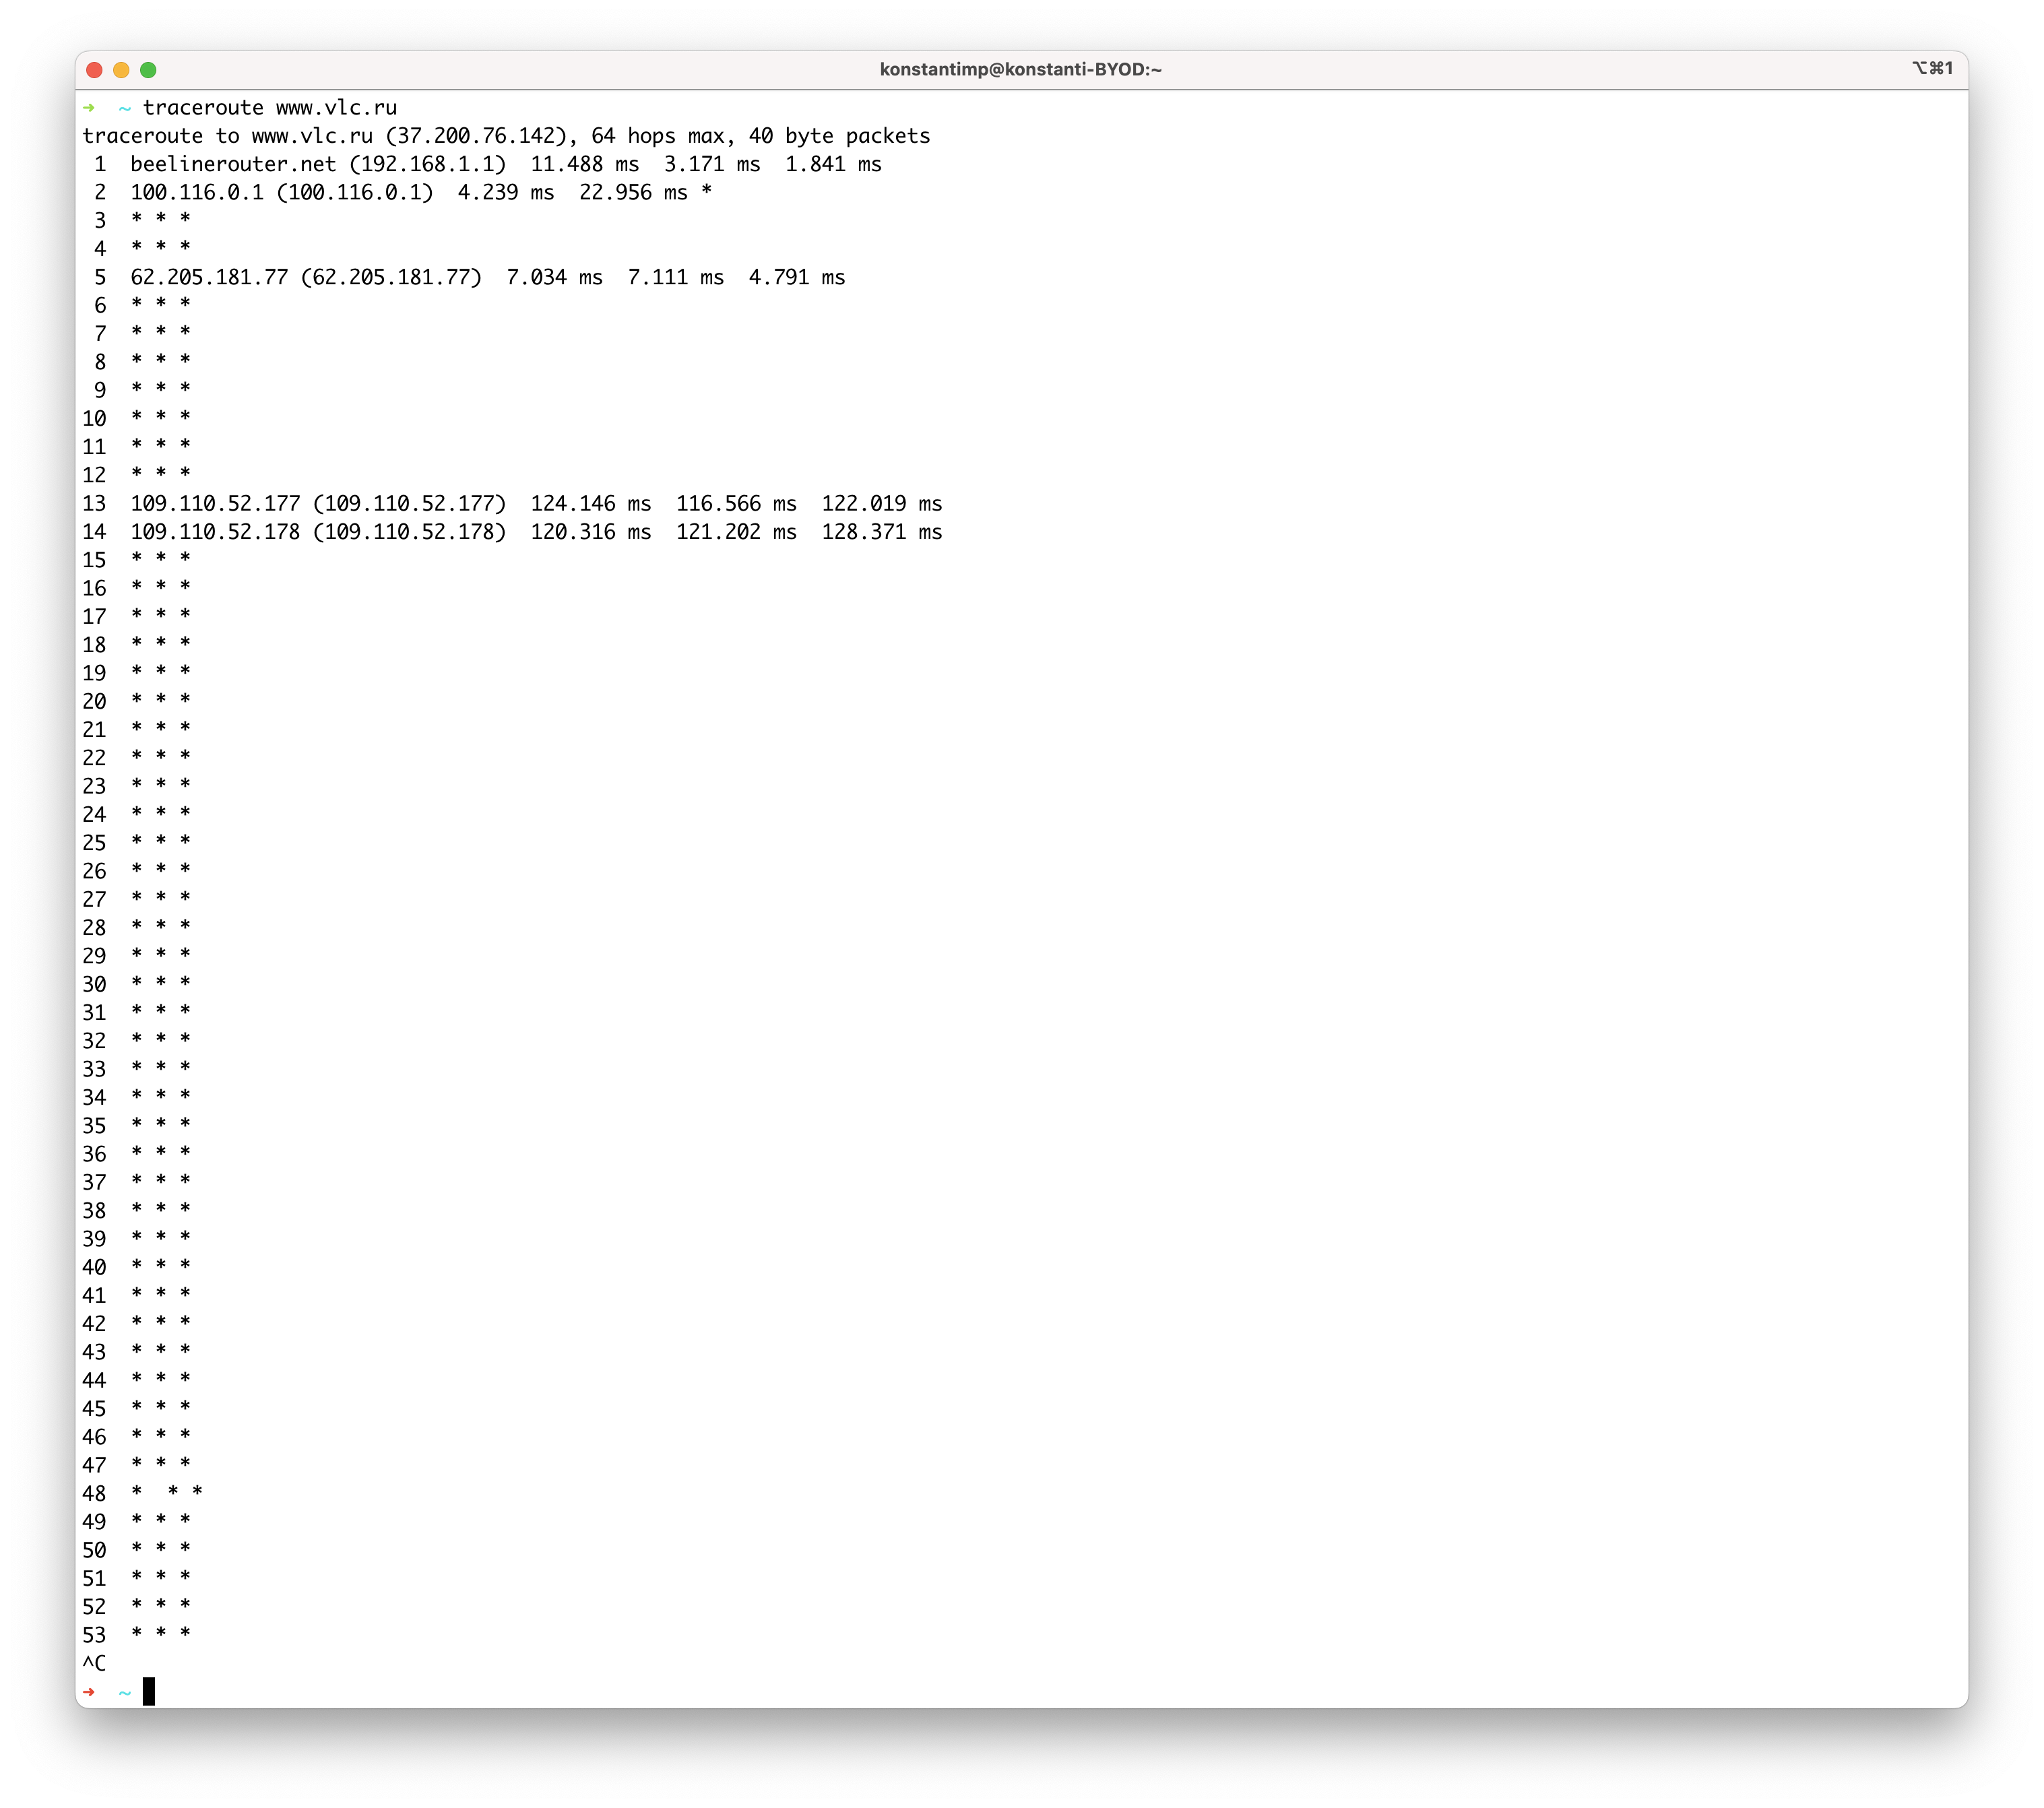
\includegraphics[width=0.8\textwidth]{s210}
    \caption{Смотрим путь пакета до \href{www.vlc.ru}{www.vlc.ru}}
  \end{figure}

  53 промежуточных хоста было, а до цели мы так и не достучались. Ви-димо, дело в том, что ping отсылает
  ICMP пакеты, а traceroute - UDP. Заставим и traceroute отправлять ICMP
  \begin{figure}[H]
    \centering
    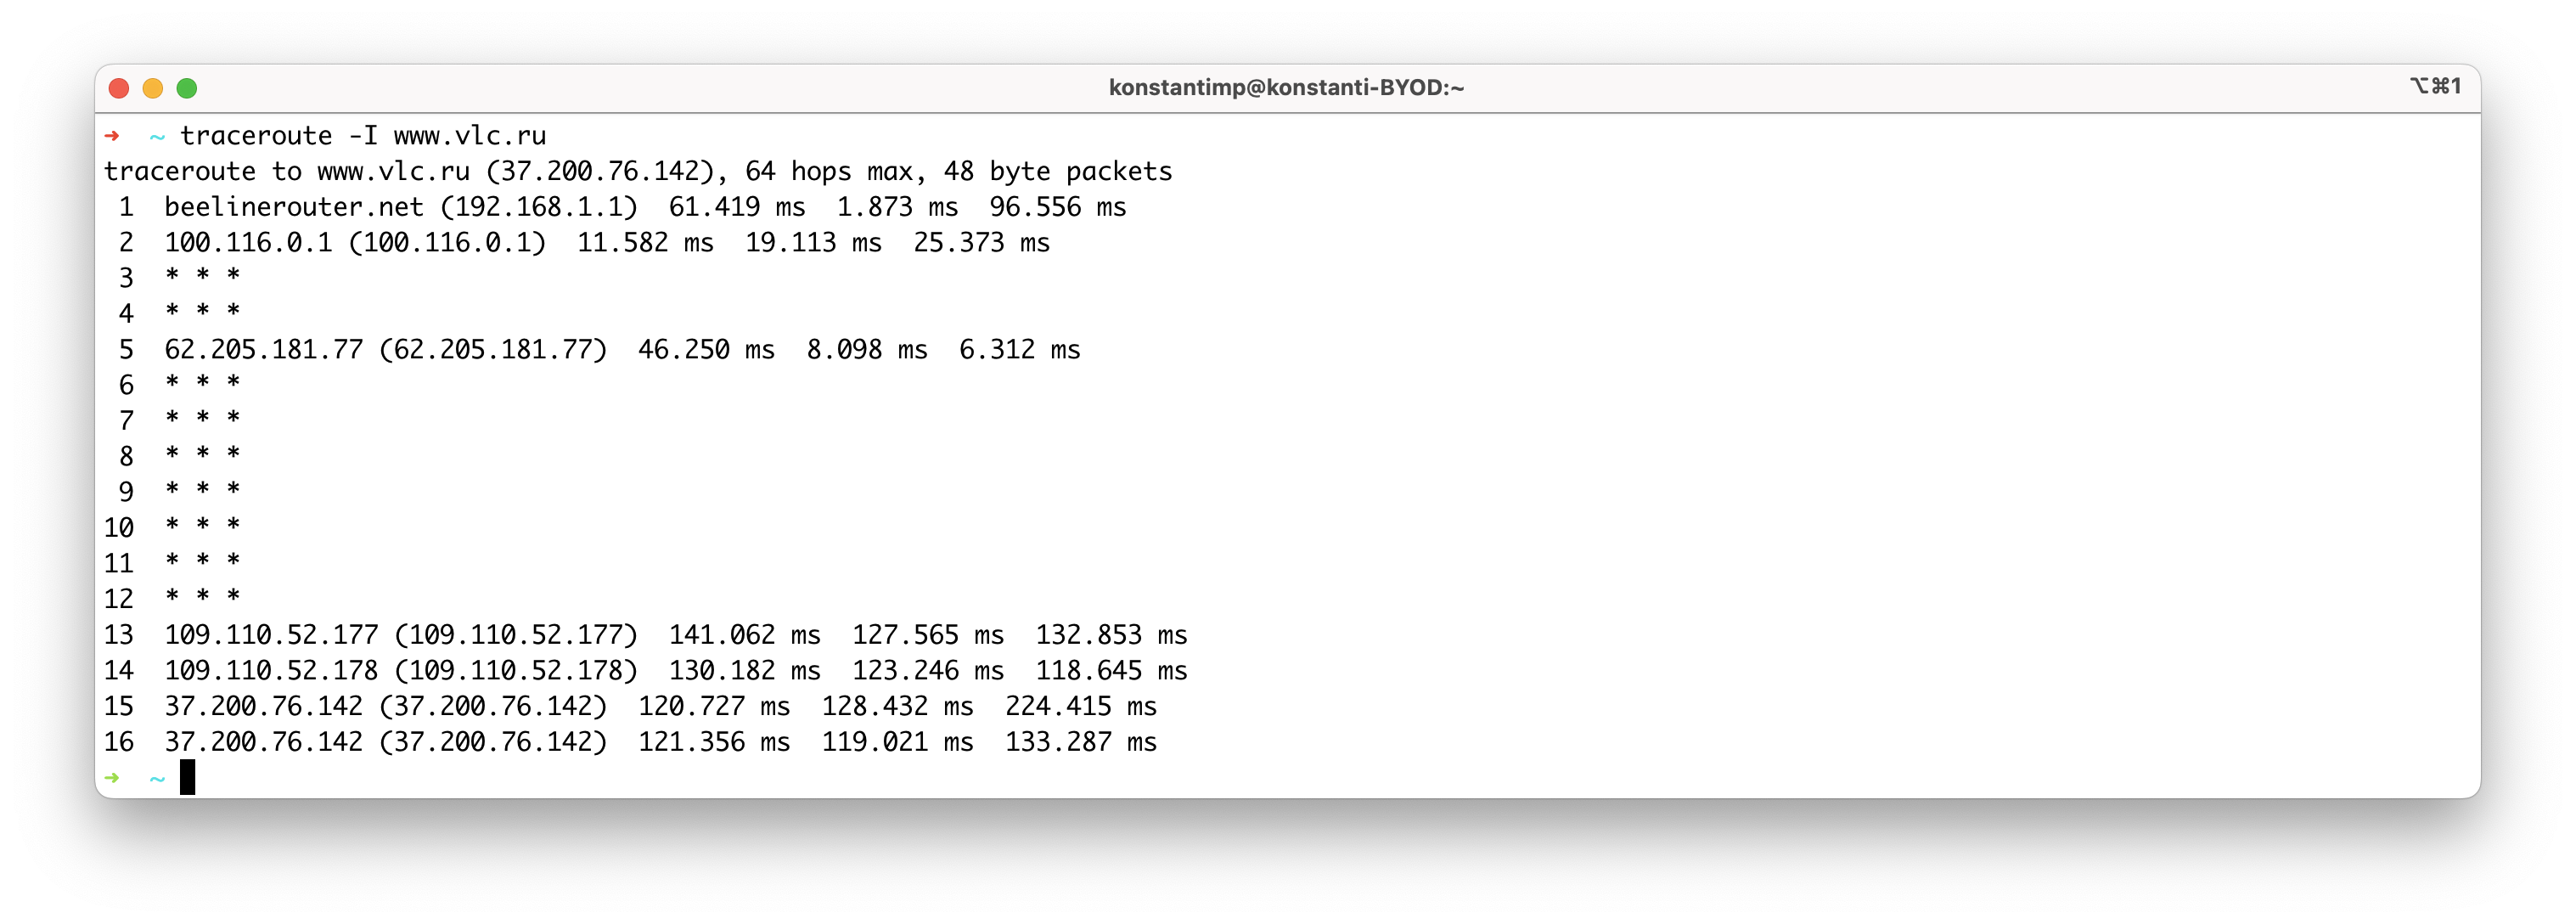
\includegraphics[width=0.8\textwidth]{s211}
    \caption{Смотрим путь ICMP пакета до \href{www.vlc.ru}{www.vlc.ru}}
  \end{figure}

  Намного лучше - 15 промежуточных хостов. Наиболее долго пакеты до-летали с 14 и 15 (они дальше, поэтому и дольше).
  
  \begin{figure}[H]
    \centering
    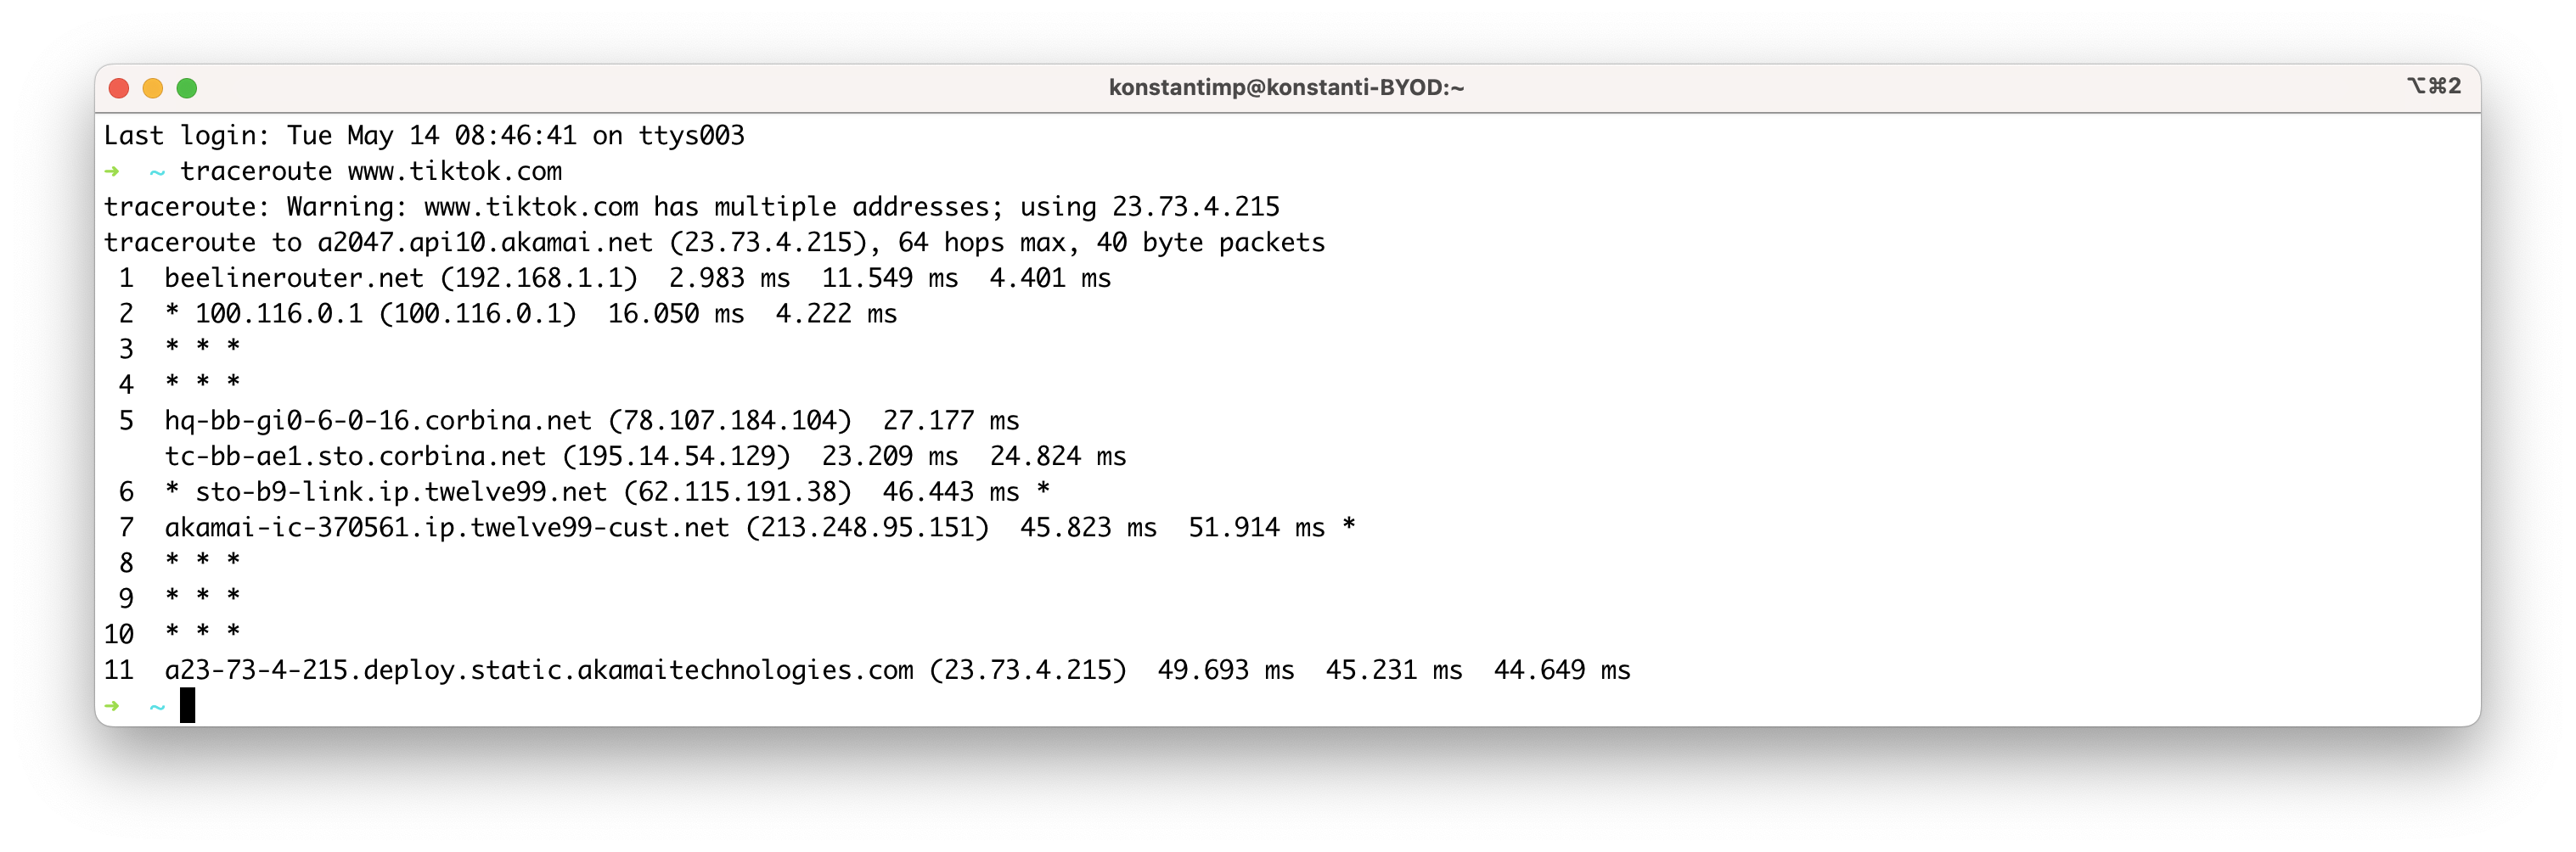
\includegraphics[width=0.8\textwidth]{s212}
    \caption{Смотрим путь пакета до \href{www.tiktok.ru}{www.tiktok.ru}}
  \end{figure}

  10 промежуточных хостов, статус наихудшего получает 7.

  \newpage
  \section{Если нет traceroute, но есть ping}

  \textbf{traceroute} отправляет пакеты на целевой хост, постепенно увеличивая TTL. Таким образом
  пакет по очереди <<умирает>> на каждой точке маршрута. Такого же эффекта мы можем добиться,
  используя руки и \textbf{ping}. Судя по выводу \textbf{traceroute} из предыдущего пунтка,
  быстрее всего будет таким образом досту-чаться до \href{opera.com}{opera.com}. Попробуем

  
  \begin{figure}[H]
    \centering
    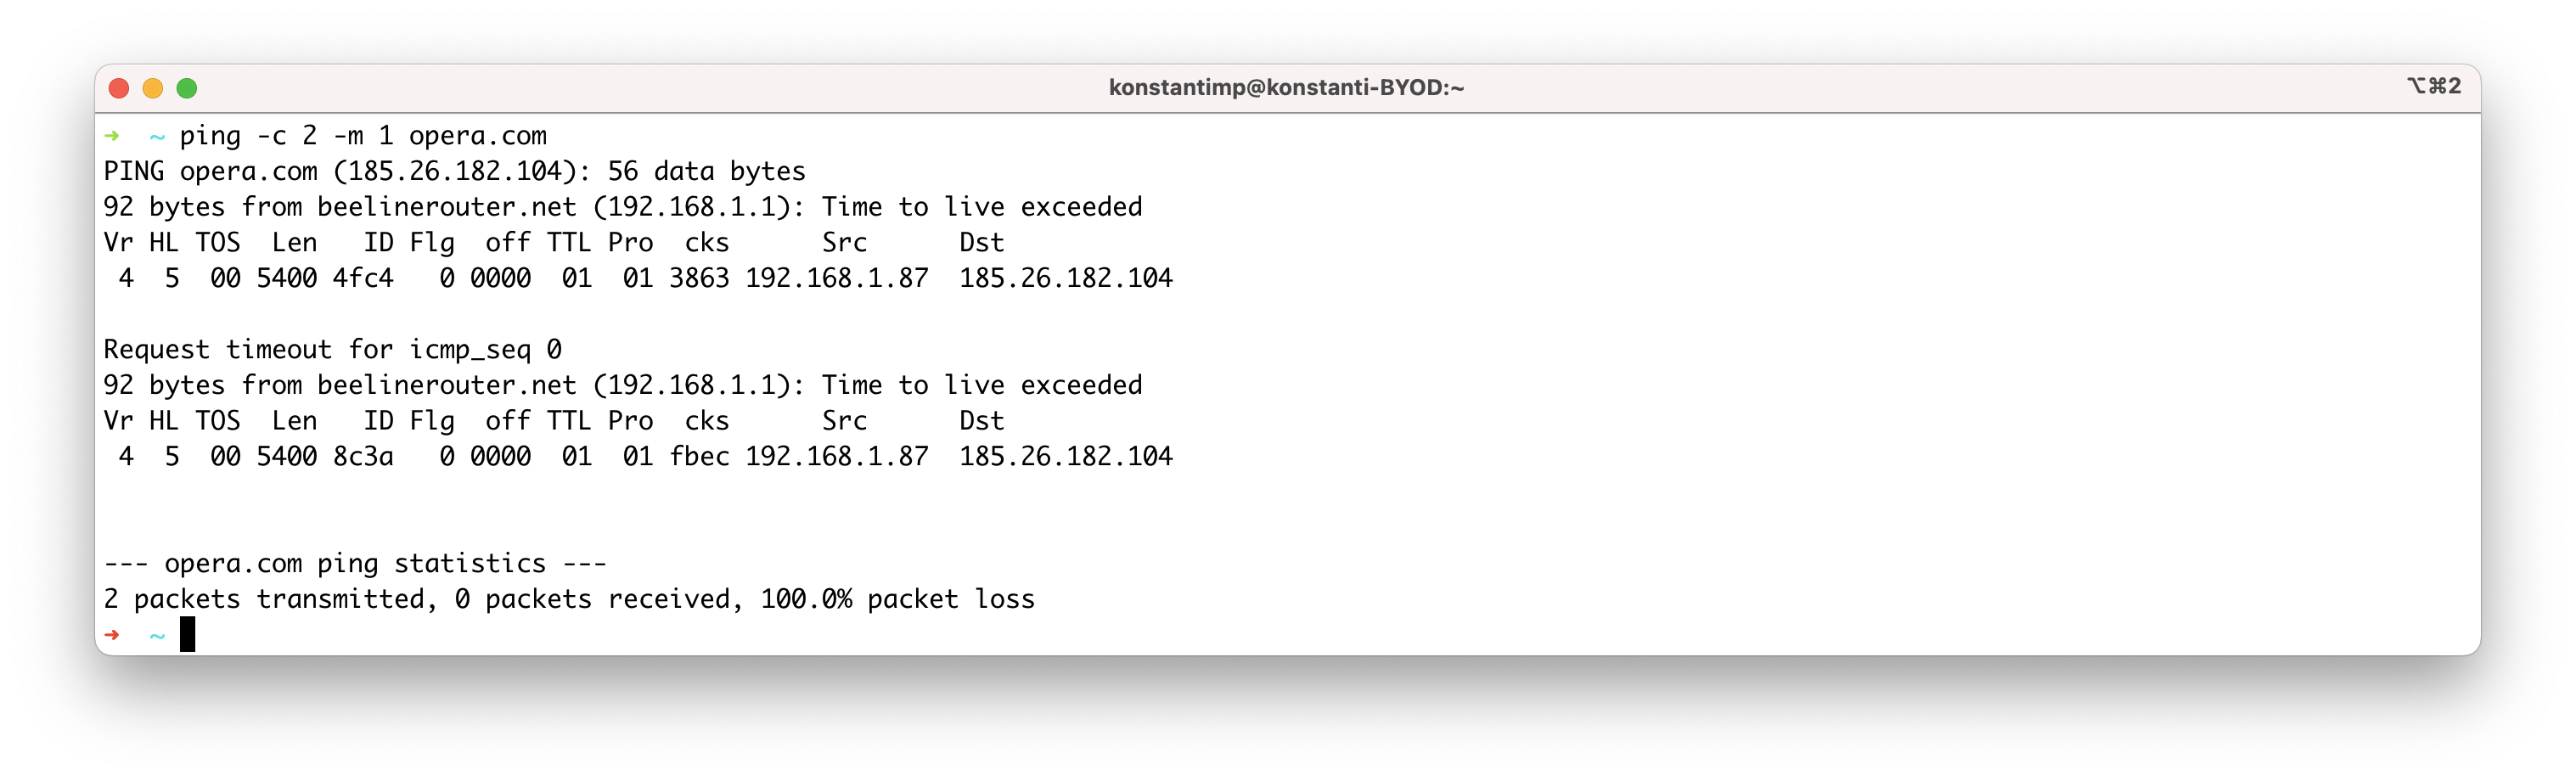
\includegraphics[width=0.8\textwidth]{s213}
    \caption{TTL = 1, exceeded}
  \end{figure}
  \begin{figure}[H]
    \centering
    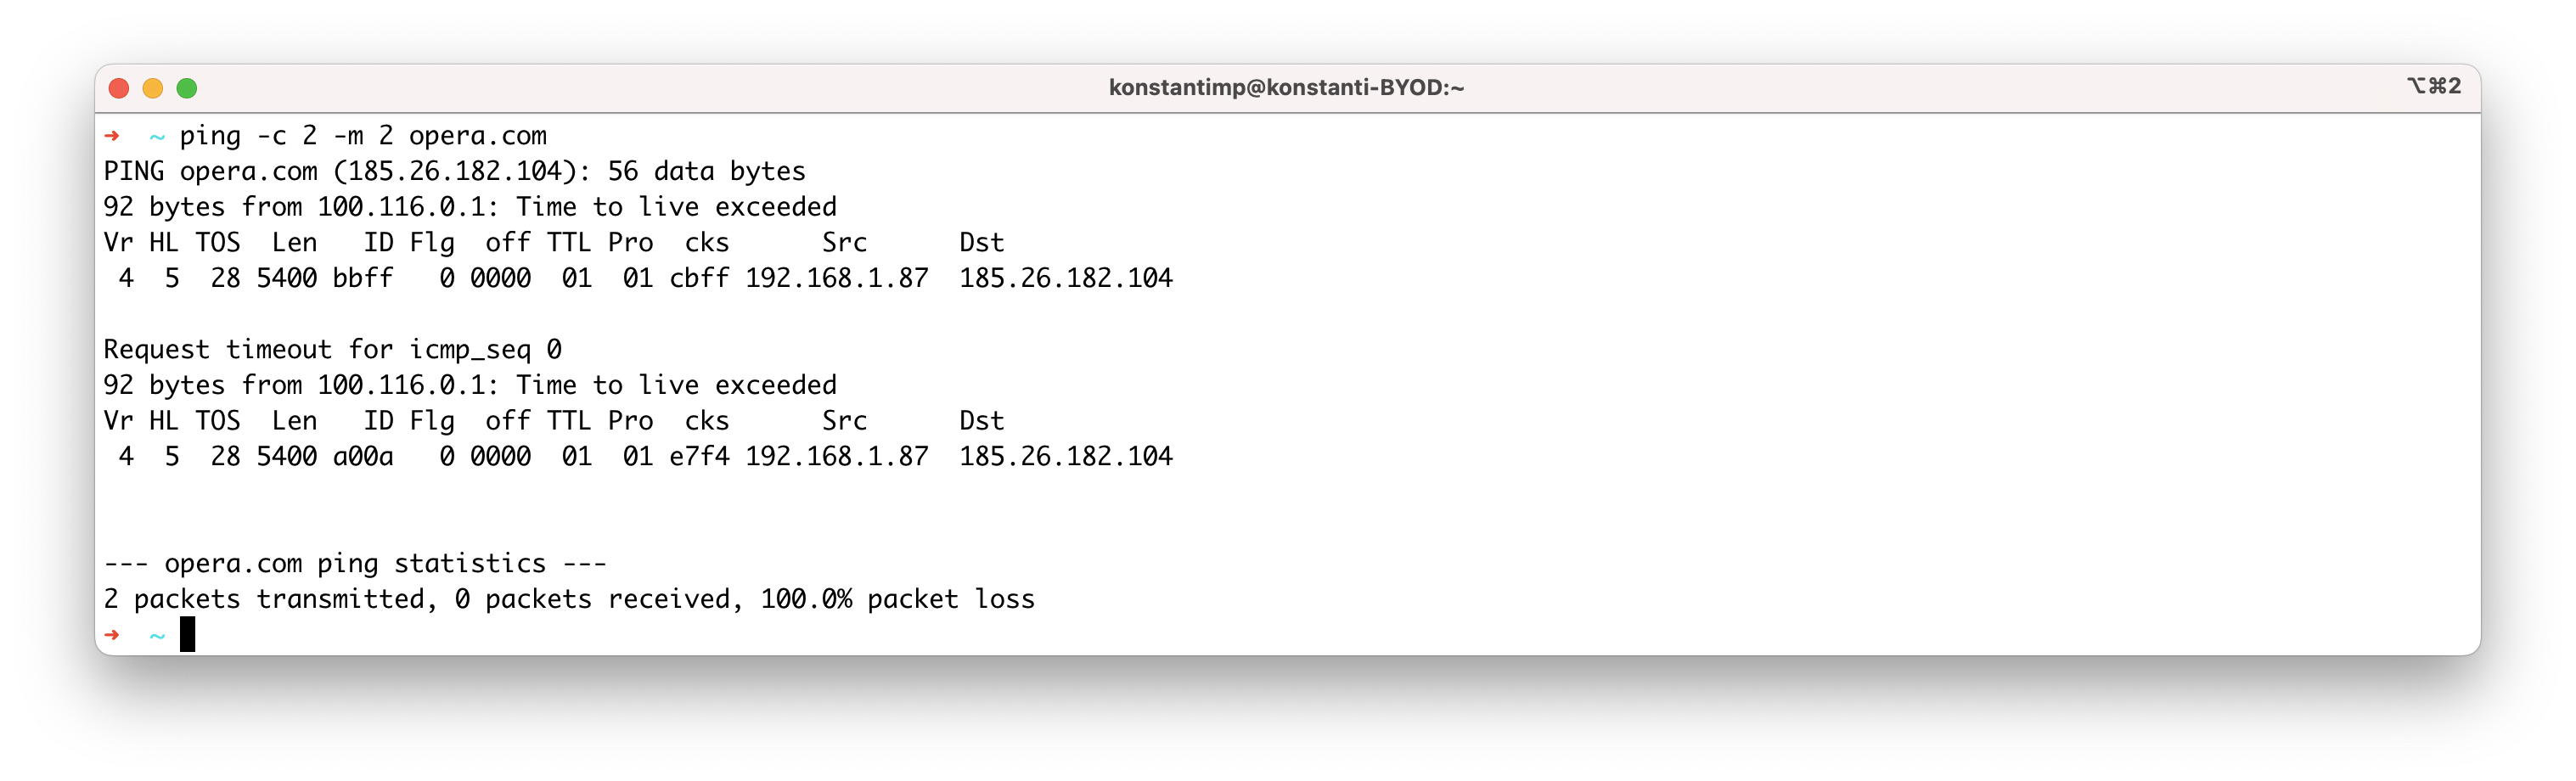
\includegraphics[width=0.8\textwidth]{s214}
    \caption{TTL = 2, exceeded}
  \end{figure}
  \begin{figure}[H]
    \centering
    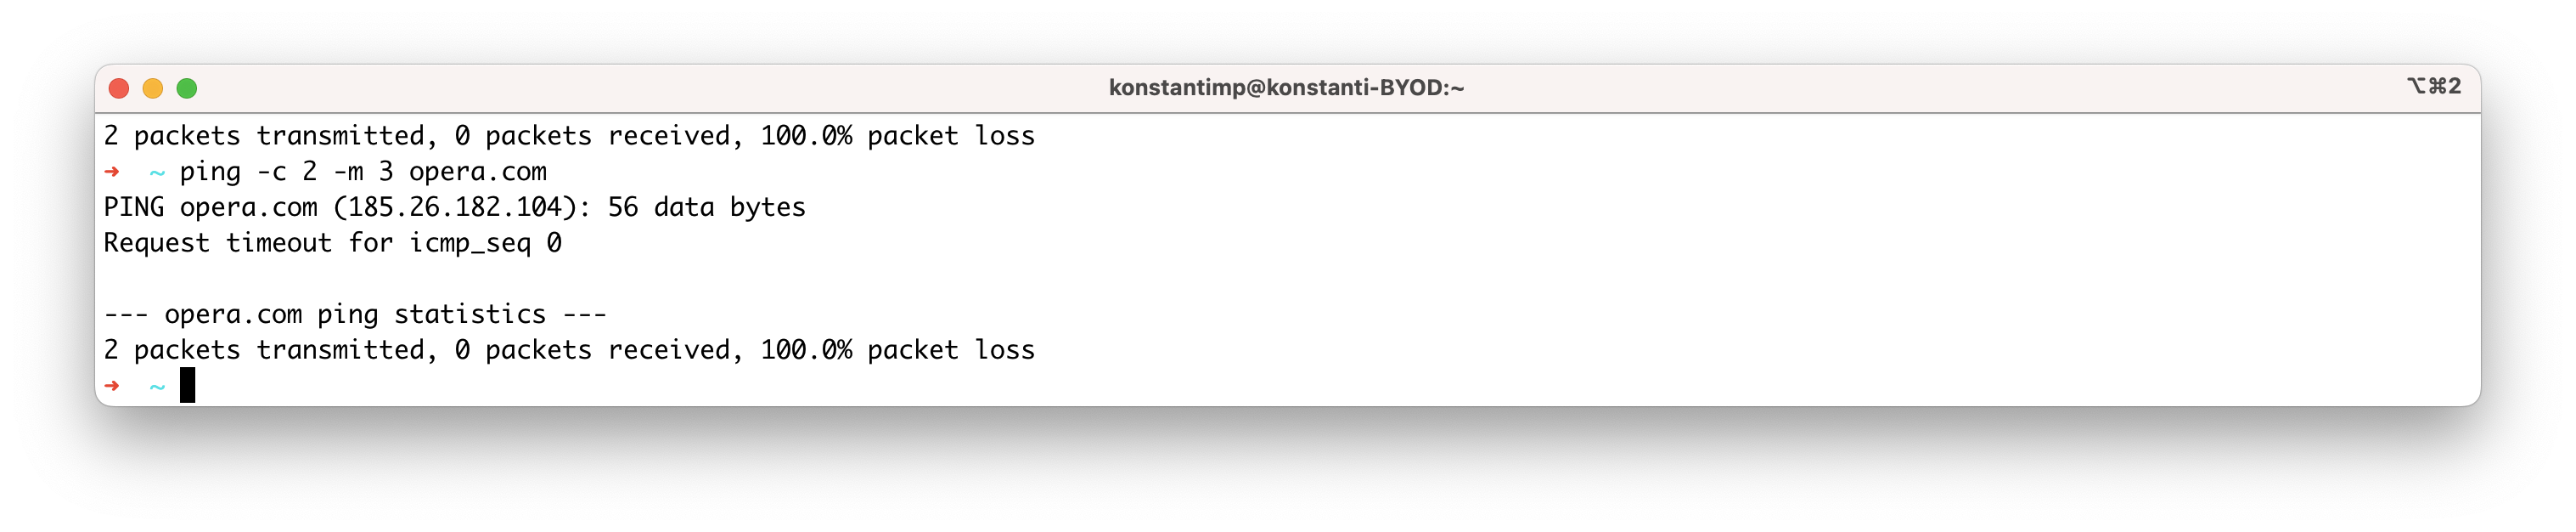
\includegraphics[width=0.8\textwidth]{s215}
    \caption{TTL = 3, exceeded}
  \end{figure}
  \begin{figure}[H]
    \centering
    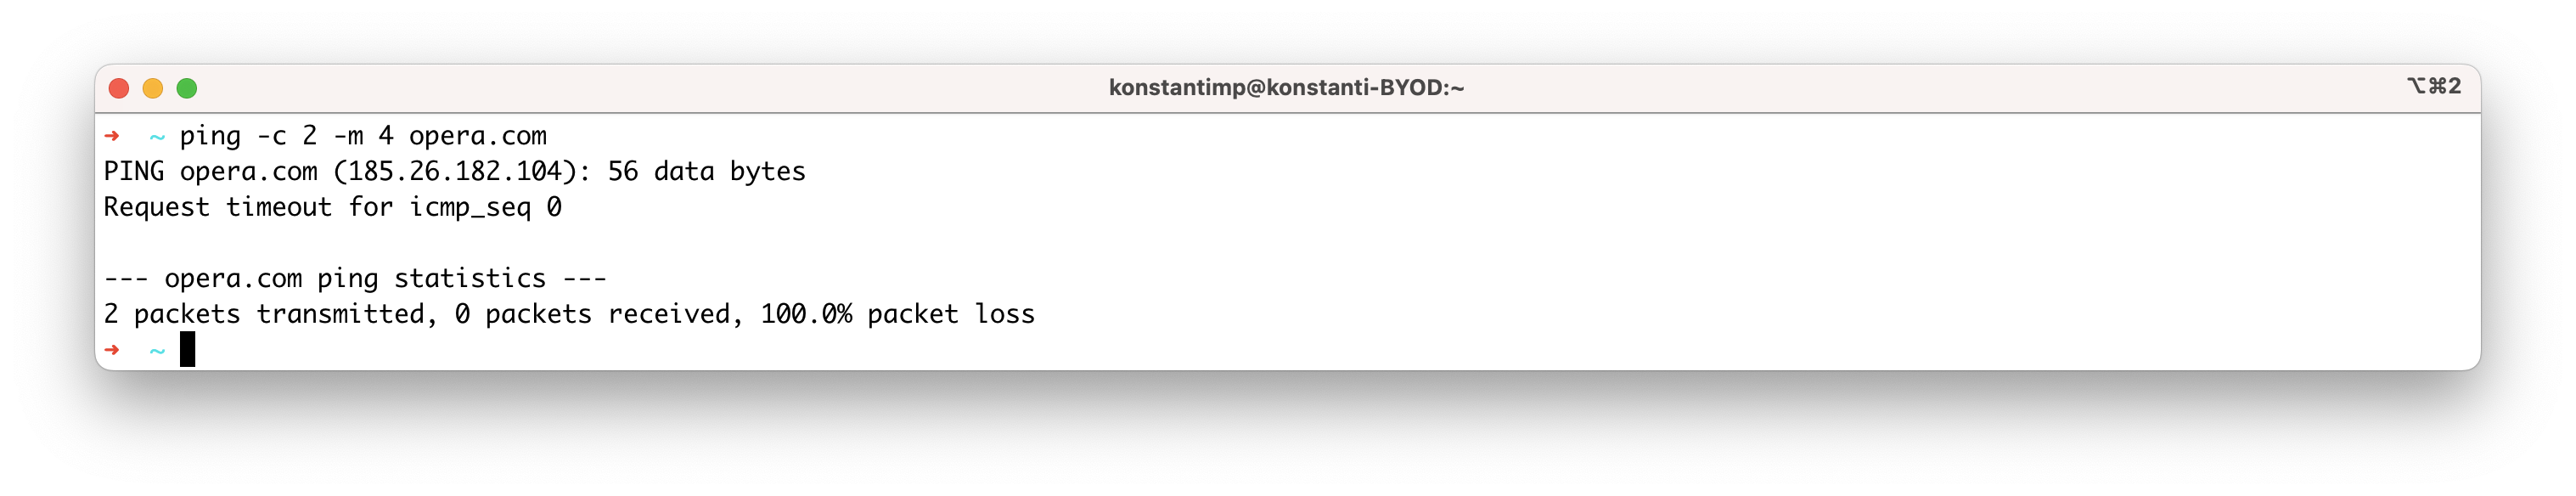
\includegraphics[width=0.8\textwidth]{s216}
    \caption{TTL = 4, exceeded}
  \end{figure}
  \begin{figure}[H]
    \centering
    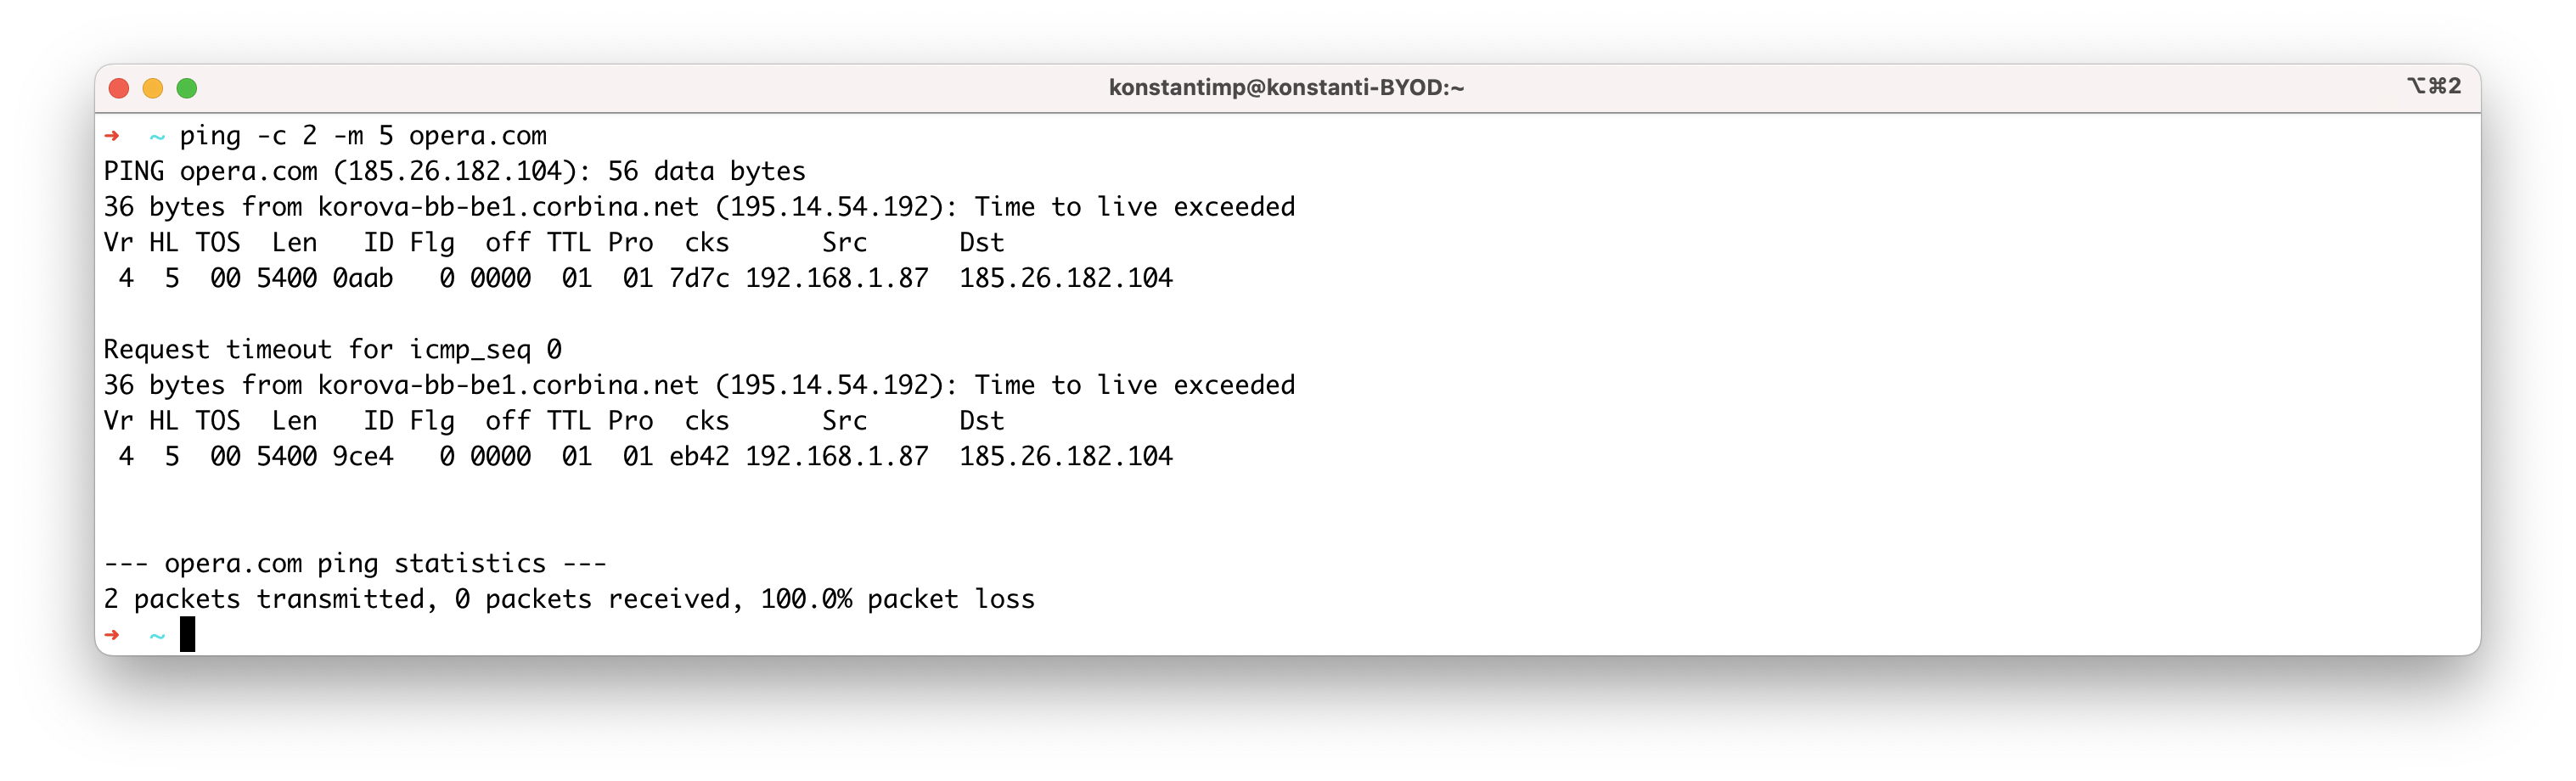
\includegraphics[width=0.8\textwidth]{s217}
    \caption{TTL = 5, exceeded}
  \end{figure}
  \begin{figure}[H]
    \centering
    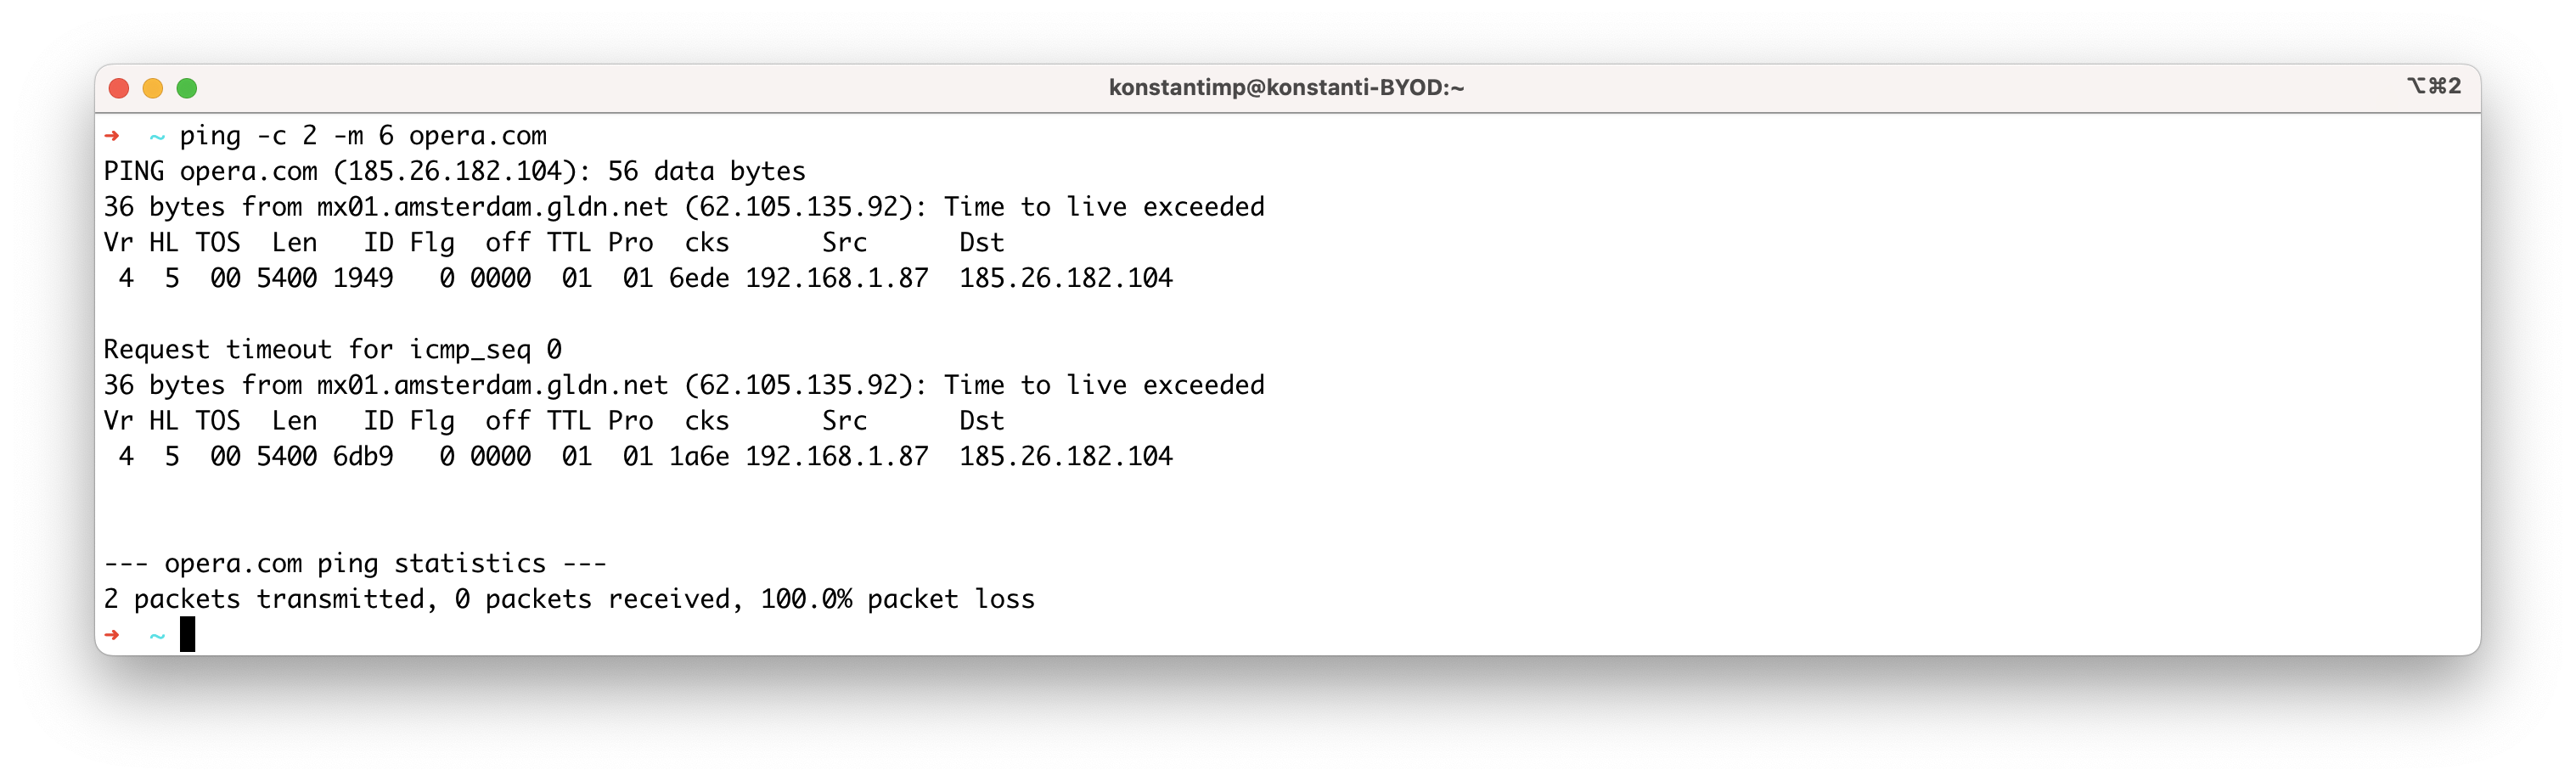
\includegraphics[width=0.8\textwidth]{s218}
    \caption{TTL = 6, exceeded}
  \end{figure}
  \begin{figure}[H]
    \centering
    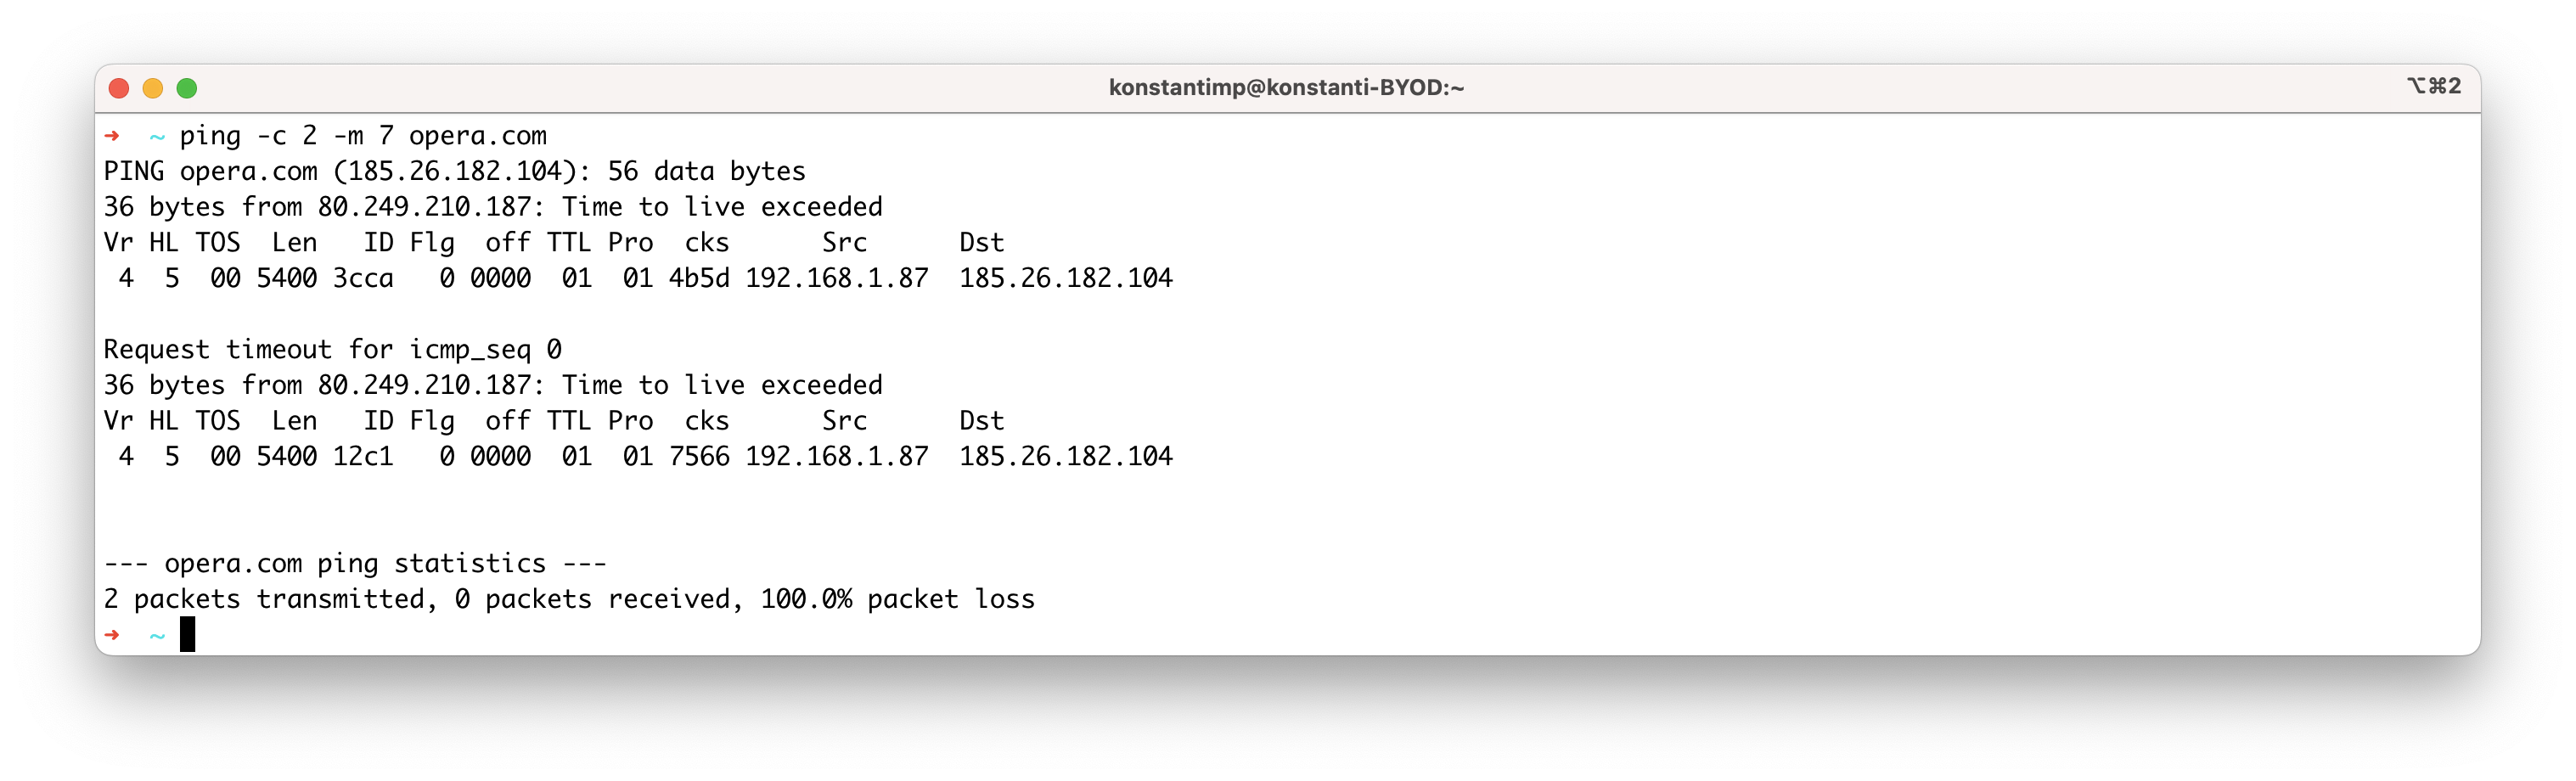
\includegraphics[width=0.8\textwidth]{s219}
    \caption{TTL = 7, exceeded}
  \end{figure}
  \begin{figure}[H]
    \centering
    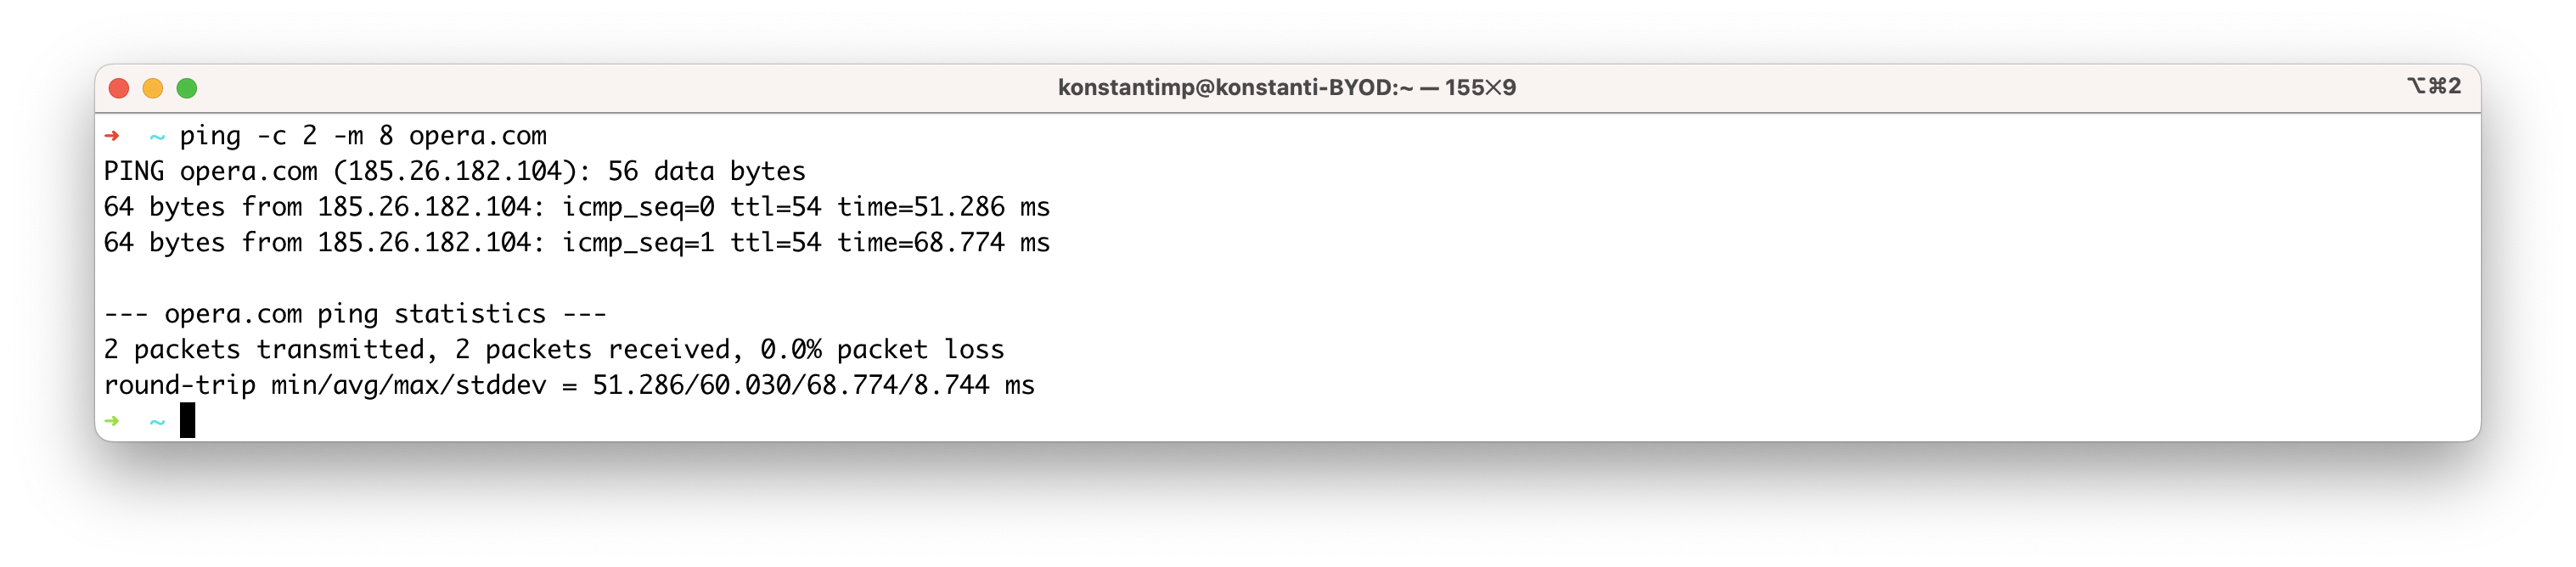
\includegraphics[width=0.8\textwidth]{s220}
    \caption{TTL = 8, reached}
  \end{figure}

  Полностью совпадает с выводом \textbf{traceroute}.

  \newpage
  \section{Если нет tracerout, но есть mtr}

  Не знаю, когда такое может быть, потому что \textbf{mtr} пришлось скачивать. Вот он
  \begin{figure}[H]
    \centering
    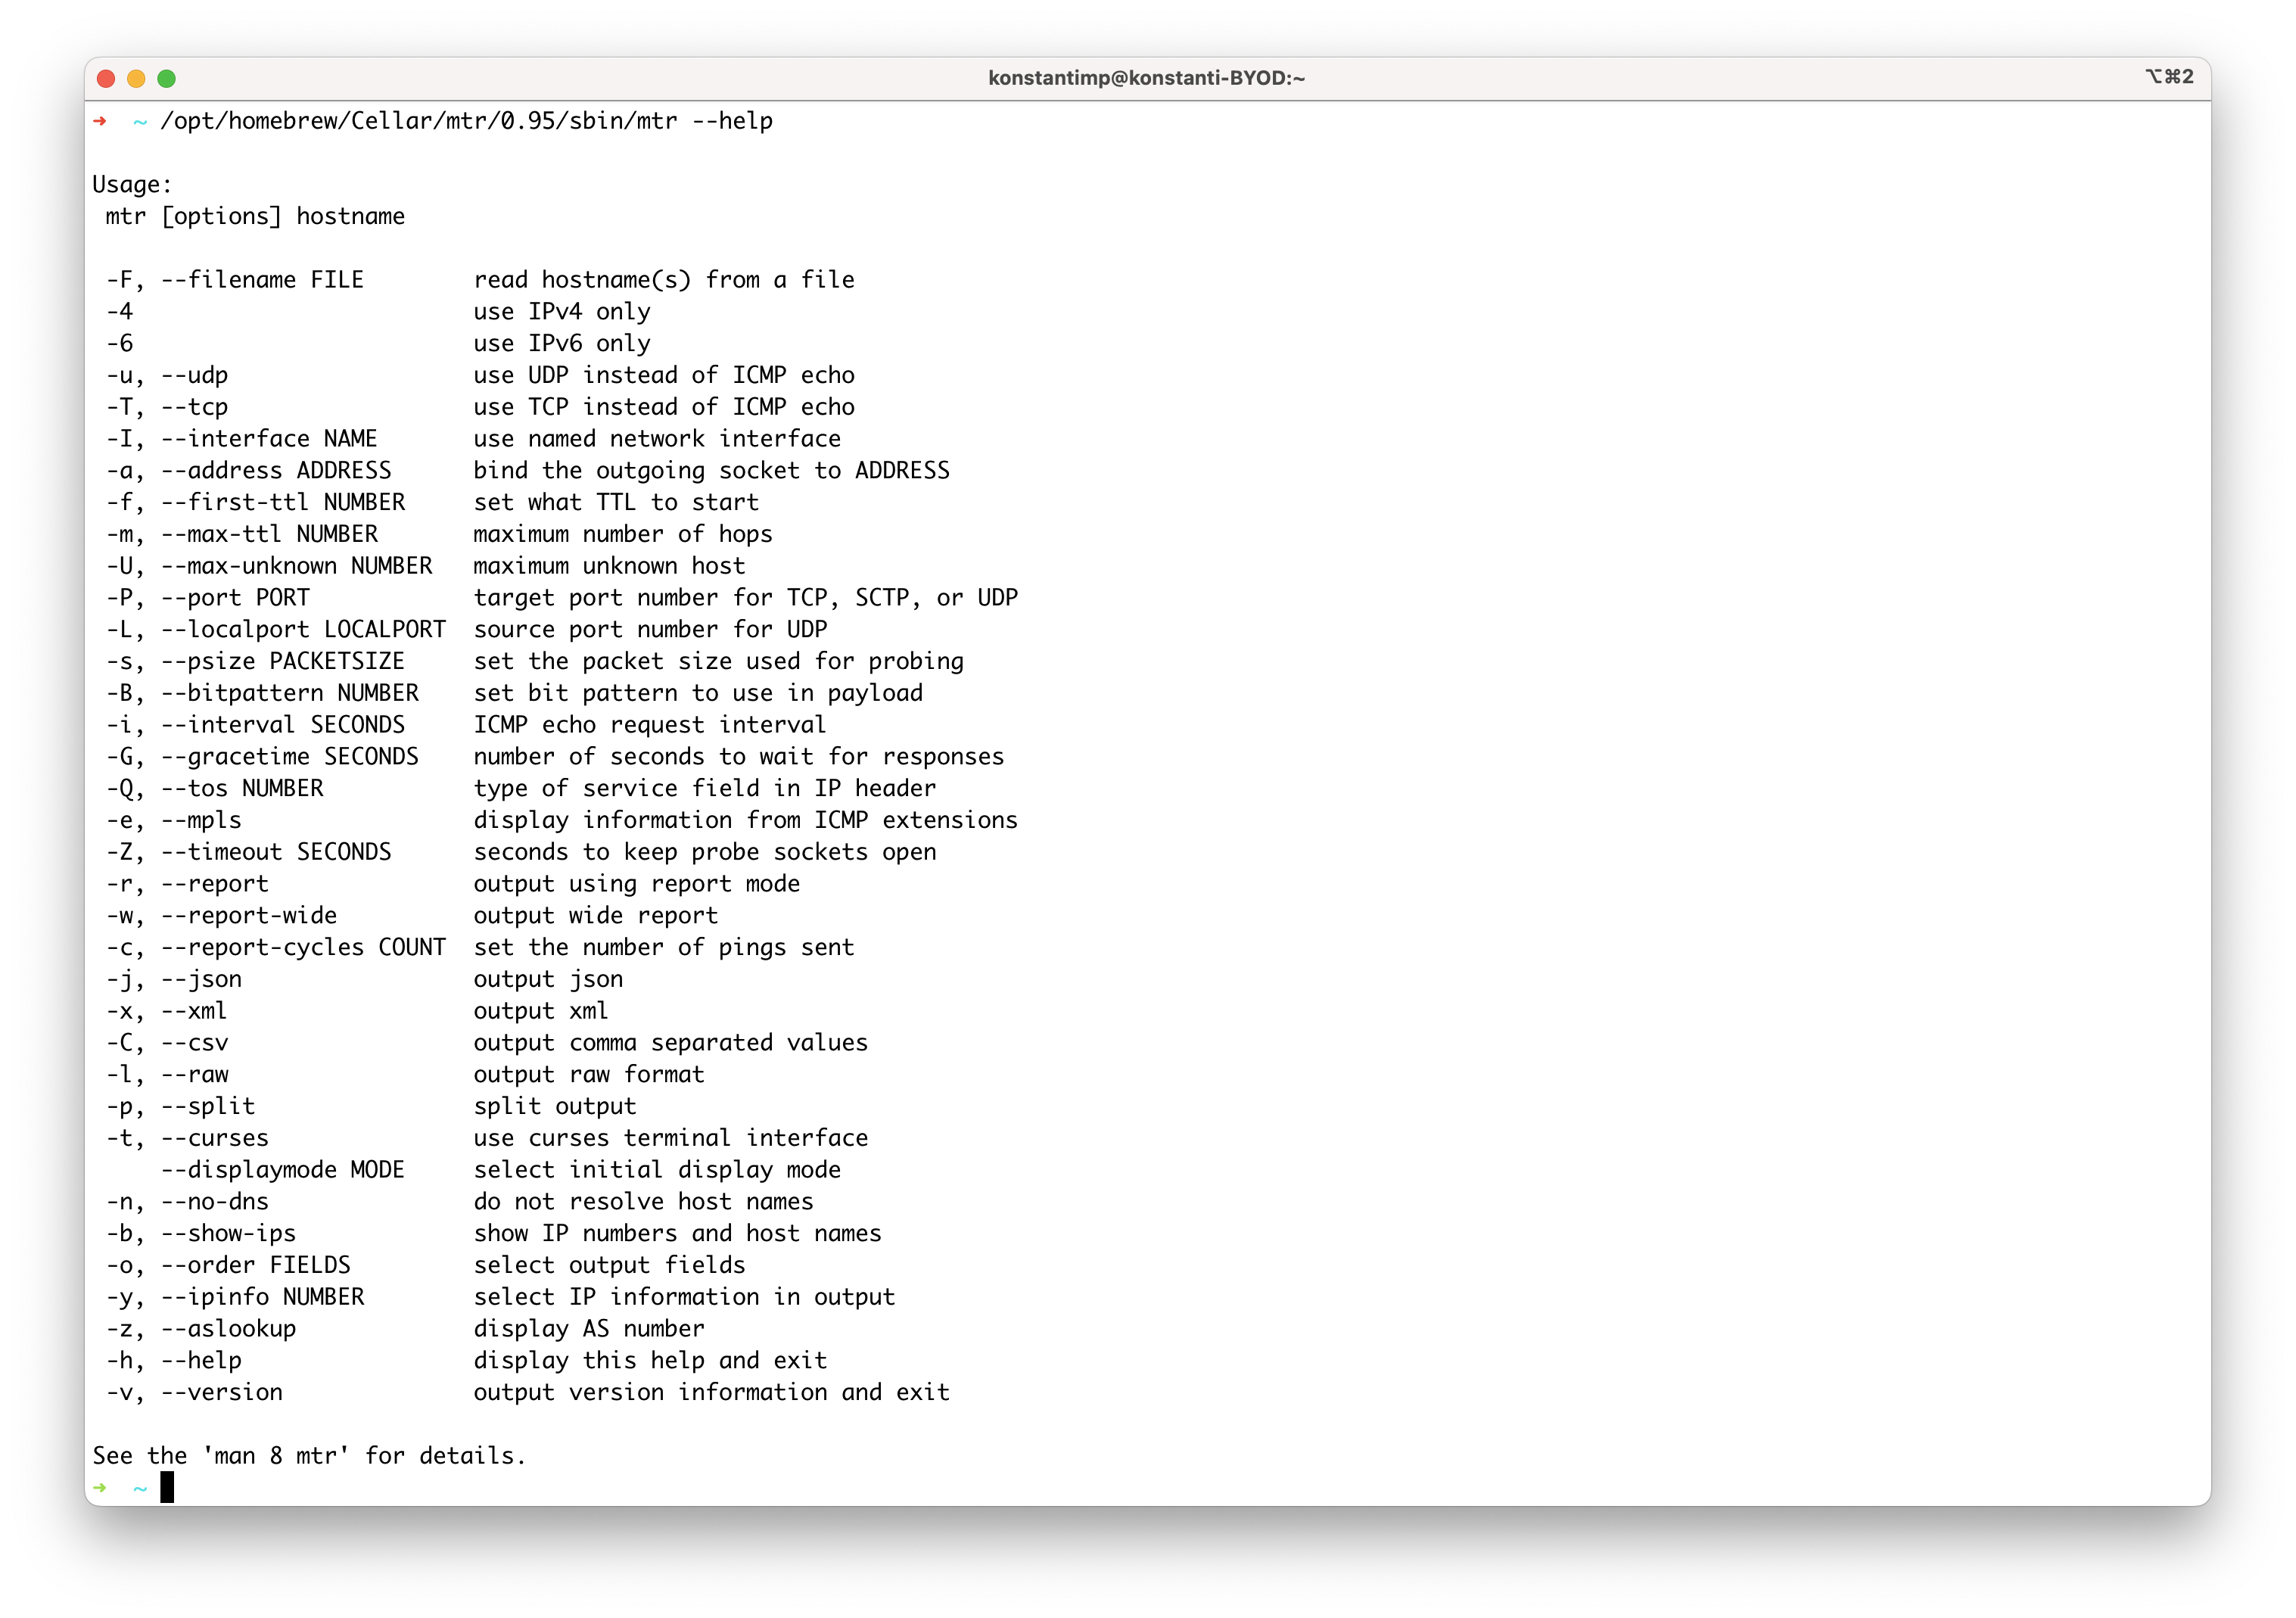
\includegraphics[width=0.8\textwidth]{s221}
    \caption{Утилита \textbf{mtr}}
  \end{figure}
  
  \begin{figure}[H]
    \centering
    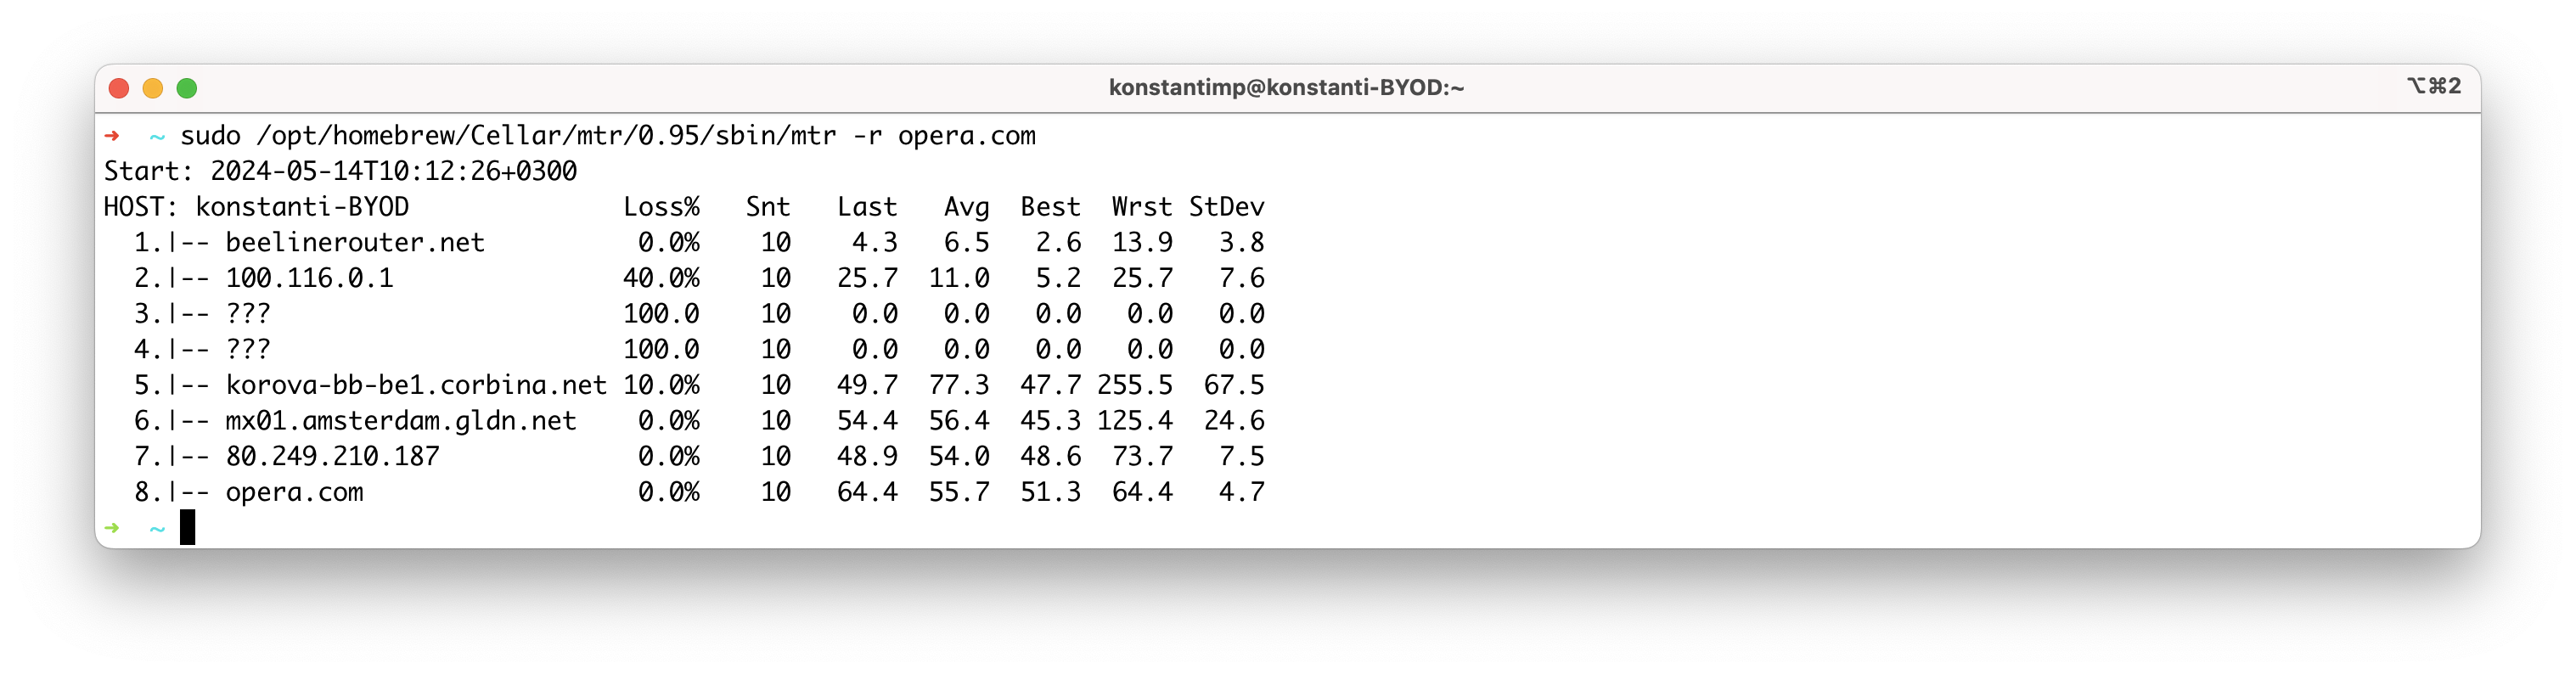
\includegraphics[width=0.8\textwidth]{s222}
    \caption{Смотрим путь до \href{opera.com}{opera.com}}
  \end{figure}

  Получен путь, полностью идентичный выводу \textbf{traceroute} и \textbf{ping}.

  \newpage
  \section{Графы}

  Теперь мы хотим картинок и устанавливаем и запускаем \textbf{tracemap}

  \begin{minted}{bash}
    wget http://xgu.ru/download/tracemap.pl
    (echo "opera.com";
      echo "www.vlc.ru";
      echo "www.tiktok.com"
    ) | perl tracemap.pl
  \end{minted}

  \begin{figure}[H]
    \centering
    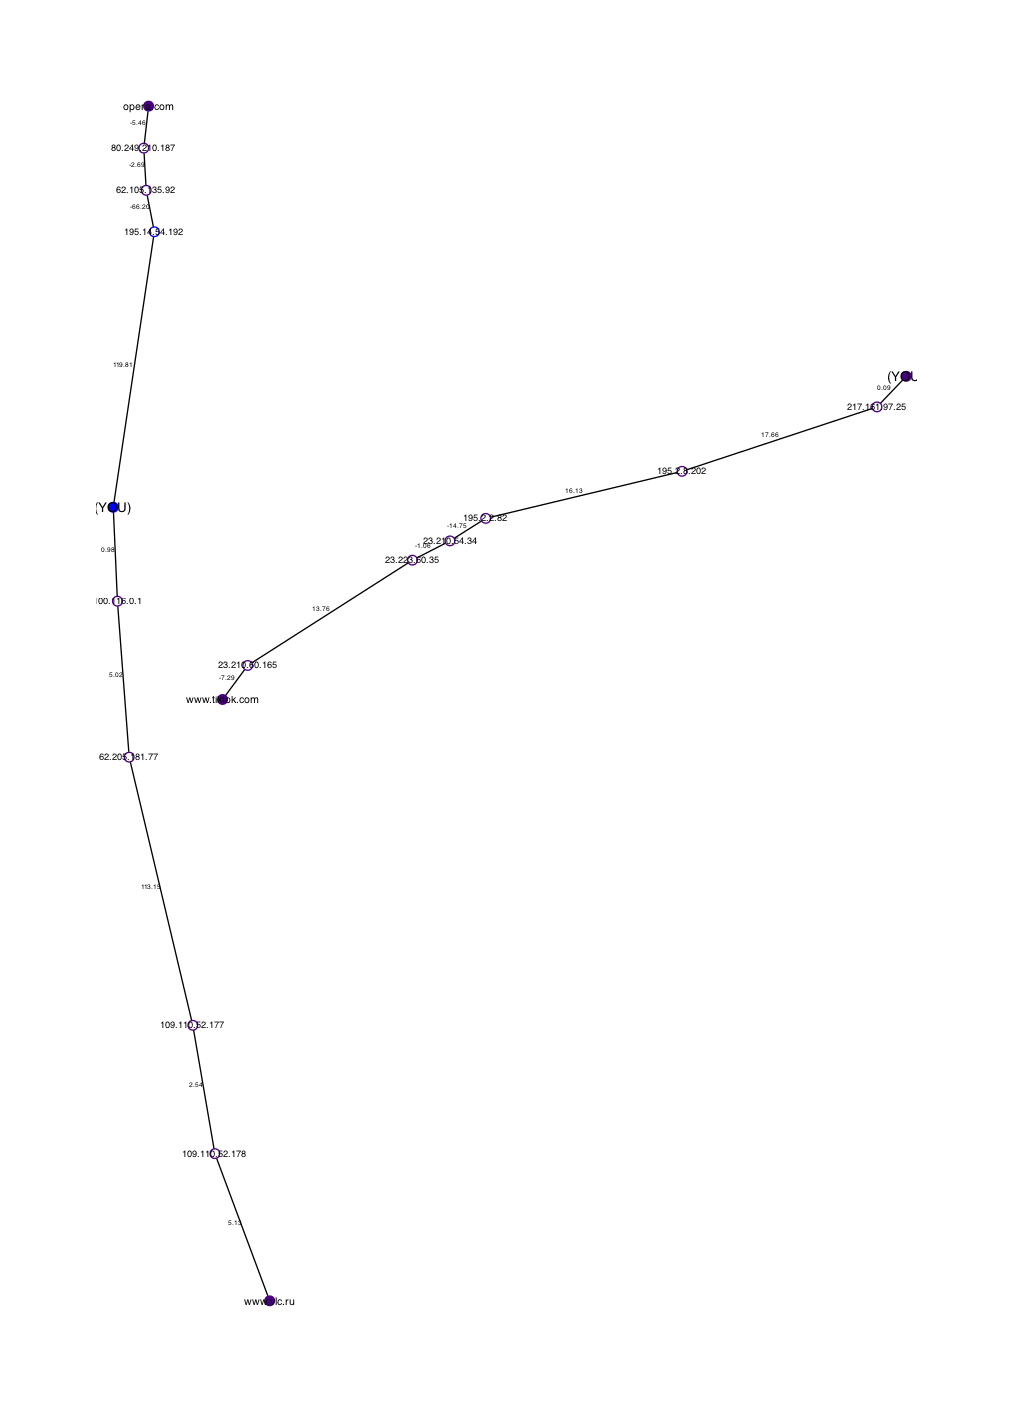
\includegraphics[width=\textwidth]{tracemap.png}
    \caption{Что из этого вышло}
  \end{figure}

\end{document}
